\subsection{(a,b)-Trees}
\subsubsection{Introduction}

\begin{frame}{(a,b)-Trees}{Introduction}
  \textbf{(a,b)-Tree:}
  \begin{itemize}
    \item<2->
      Also known as \textbf{b-tree} (b for \enquote{balanced})
    \item<3->
      Used in databases and file systems
  \end{itemize}
  \onslide<4->
  \textbf{Idea:}
  \begin{itemize}
    \item<5->
      Save a varying number of elements per node
    \item<6->
      So we have space for elements on an \texttt{\color{MainA}insert}
      and balance operation
  \end{itemize}
\end{frame}

%-------------------------------------------------------------------------------

\begin{frame}{(a,b)-Trees}{Introduction}
  \textbf{(a,b)-Tree:}
  \begin{itemize}
    \item<2->
      All leaves have the same depth
    \item<3->
      Each inner node has {\color{MainA}$\geq a$} and
      {\color{MainA}$\leq b$} nodes\\
      (Only the root node may have less nodes)
  \end{itemize}
  \onslide<4->
  \begin{figure}
    \begin{adjustbox}{width=0.3\linewidth}
      \begin{tikzpicture}[
  node/.style={
    rectangle,
    color=black,
    draw=Mittel-Blau,
    fill=Hell-Blau,
    line width=0.15em,
    minimum size=2.0em,
    inner sep=0em
  }, path_start/.style={
%    -{Computer Modern Rightarrow[length=0.5em]},
    -{Stealth[length=1.25em]},
    line width=0.25em,
    color=Mittel-Gruen
  }, path/.style={
    path_start,
%    {Circle[scale=0.5,round]}-{Computer Modern Rightarrow[length=0.5em]},
    {Circle[scale=0.5,round]}-{Stealth[length=1.25em]},
    shorten <=-0.35em
  }, level/.style={
    sibling distance=0.0em,
    level distance=3.0em
  }]
\node [node, xshift=-2em] {2}
child [path, xshift=-3em, edge from parent path={
  (\tikzparentnode.south west) -- (\tikzchildnode.north)}
] { };

\node [node] {10}
child [path, xshift=-2em, edge from parent path={
  (\tikzparentnode.south west) -- (\tikzchildnode.north)}
] { };

\node [node, xshift=2em] {18}
child [path, xshift=0em, edge from parent path={
  (\tikzparentnode.south west) -- (\tikzchildnode.north)}
] { }
child [path, xshift=3em, edge from parent path={
  (\tikzparentnode.south east) -- (\tikzchildnode.north)}
] { };
\end{tikzpicture}
    \end{adjustbox}
    \label{fig:a_b_tree:node_introduction}
  \end{figure}
    \begin{itemize}
    \item<5->
      Each node with {\color{MainA}$n$} children is called \enquote{node of degree $n$} and
      holds {\color{MainA}$n-1$} sorted elements
    \item<6->
      Subtrees are located \enquote{between} the elements
    \item<7->
      We require: {\color{MainA}$a \geq 2$} and
      {\color{MainA}$b \geq 2\,a - 1$}
  \end{itemize}
\end{frame}

%-------------------------------------------------------------------------------

\begin{frame}{(a,b)-Trees}{Introduction}
  \textbf{(2,4)-Tree:}
    \begin{figure}
    \begin{adjustbox}{width=0.75\linewidth}
      \begin{tikzpicture}[
  node/.style={
    rectangle,
    color=black,
    draw=Mittel-Blau,
    fill=Hell-Blau,
    line width=0.15em,
    minimum size=2.0em,
    inner sep=0em
  }, path_start/.style={
%    -{Computer Modern Rightarrow[length=0.5em]},
    -{Stealth[length=1.25em]},
    line width=0.25em,
    color=Mittel-Gruen
  }, path/.style={
    path_start,
%    {Circle[scale=0.5,round]}-{Computer Modern Rightarrow[length=0.5em]},
    {Circle[scale=0.5,round]}-{Stealth[length=1.25em]},
    shorten <=-0.35em
  }, level/.style={
    sibling distance=0.0em,
    level distance=5.0em
  }]
\node [node] {23}
child [path, xshift=-5em, edge from parent path={
  (\tikzparentnode.south west) -- (node1.north)}
] {
  node [node, xshift=-2em] {2}
  child [path, xshift=-7.5em, edge from parent path={
    (\tikzparentnode.south west) -- (\tikzchildnode.north)}
  ] {
    node [node] {1}
  }
  node [node] (node1) {10}
  child [path, xshift=-4.5em, edge from parent path={
    (\tikzparentnode.south west) -- (node2.north)}
  ] {
    node [node, xshift=-2em] {3}
    node [node] (node2) {5}
    node [node, xshift=2em] {9}
  }
  node [node, xshift=2em] {18}
  child [path, xshift=-1.5em, edge from parent path={
    (\tikzparentnode.south west) -- (\tikzchildnode.north)}
  ] {
    node [node] {15}
  }
  child [path, xshift=1.5em, edge from parent path={
    (\tikzparentnode.south east) -- (node4.north east)}
  ] {
    node [node] (node4) {20}
    node [node, xshift=2em] {22}
  }
}
child [path, xshift=6em, edge from parent path={
  (\tikzparentnode.south east) -- (node5.north east)}
] {
  node [node, xshift=-1em] (node5) {25}
  child [path, xshift=-1.5em, edge from parent path={
    (\tikzparentnode.south west) -- (\tikzchildnode.north)}
  ] {
    node [node] {24}
  }
  node [node, xshift=1em] {33}
  child [path, xshift=-0.5em, edge from parent path={
    (\tikzparentnode.south west) -- (\tikzchildnode.north)}
  ] {
    node [node] {27}
  }
  child [path, xshift=2.5em, edge from parent path={
    (\tikzparentnode.south east) -- (node6.north east)}
  ] {
    node [node] (node6) {37}
    node [node, xshift=2em] {42}
  }
};
\end{tikzpicture}
    \end{adjustbox}
    \caption{Example of an (2,4)-tree}
    \label{fig:a_b_tree:tree_introduction}
    \end{figure}
   \vspace{-1.0em}
  \begin{itemize}
    \item<2->
      (2,4)-tree with depth of 3
    \item<3->
      Each node has between 2 and 4 children (1 to 3 elements)
  \end{itemize}
\end{frame}

%-------------------------------------------------------------------------------

\begin{frame}{(a,b)-Trees}{Introduction}
  \textbf{Not an (2,4)-Tree:}
   \begin{figure}
    \begin{adjustbox}{width=0.5\linewidth}
      \begin{tikzpicture}[
  node/.style={
    rectangle,
    color=black,
    draw=Mittel-Blau,
    fill=Hell-Blau,
    line width=0.15em,
    minimum size=2.0em,
    inner sep=0em
  }, path_start/.style={
%    -{Computer Modern Rightarrow[length=0.5em]},
    -{Stealth[length=1.25em]},
    line width=0.25em,
    color=Mittel-Gruen
  }, path/.style={
    path_start,
%    {Circle[scale=0.5,round]}-{Computer Modern Rightarrow[length=0.5em]},
    {Circle[scale=0.5,round]}-{Stealth[length=1.25em]},
    shorten <=-0.35em
  }, level/.style={
    sibling distance=0.0em,
    level distance=5.0em
  }]
\node [node] {23}
child [path, xshift=-5em, edge from parent path={
  (\tikzparentnode.south west) -- (node1.north east)}
] {
  node [node, xshift=-2em] {2}
  child [path, xshift=-5.5em, edge from parent path={
    (\tikzparentnode.south west) -- (\tikzchildnode.north)}
  ] {
    node [node] {1}
    child [path, xshift=-1.5em, edge from parent path={
      (\tikzparentnode.south west) -- (\tikzchildnode.north)}
    ] {
      node [node] {0}
    }
    child [path, xshift=1.5em, edge from parent path={
      (\tikzparentnode.south east) -- (\tikzchildnode.north)}
    ] {
      node [node] {3}
    }
  }
  node [node] (node1) {18}
  child [path, xshift=-4.5em, edge from parent path={
    (\tikzparentnode.south west) -- (node2.north east)}
  ] {
    node [node] (node2) {5}
    node [node, xshift=2em] {9}
  }
  node [node, xshift=2em] {10}
  child [path, xshift=-1.5em, edge from parent path={
    (\tikzparentnode.south west) -- (\tikzchildnode.north)}
  ] {
    node [node] {15}
  }
  node [node, xshift=4em] {24}
  child [path, xshift=-0.5em, edge from parent path={
    (\tikzparentnode.south west) -- (node4.north east)}
  ] {
    node [node] (node4) {20}
    node [node, xshift=2em] {22}
  }
  child [path, xshift=4.5em, edge from parent path={
    (\tikzparentnode.south east) -- (\tikzchildnode.north)}
  ] {
    node [node] {25}
  }
}
child [path, xshift=6em, edge from parent path={
  (\tikzparentnode.south east) -- (\tikzchildnode.north)}
] {
  node [node] (node5) {33}
  child [path, xshift=0.5em, edge from parent path={
    (\tikzparentnode.south west) -- (\tikzchildnode.north)}
  ] {
    node [node] {27}
  }
};
\end{tikzpicture}
    \end{adjustbox}
    \caption{\textbf{Not} an (2,4)-tree}
    \label{fig:a_b_tree:tree_invalid_introduction}
   \end{figure}
  \vspace{-1.0em}
  \begin{itemize}
    \item<2->
      Invalid sorting
    \item<3->
      Degree of node too large / too small
    \item<4->
      Leaves on different levels
  \end{itemize}
\end{frame}

%-------------------------------------------------------------------------------

\begin{frame}{(a,b)-Trees}{Implementation - Lookup}
  \textbf{Searching an element:} (\texttt{\color{MainA}lookup})
  \begin{itemize}
    \item<2->
      The same algorithm as in {\color{MainA}BinarySearchTree}
    \item<3->
      Searching from the root downwards
    \item<4->
      The keys at each node set the path
  \end{itemize}
  \onslide<5->
  \begin{figure}[!h]
    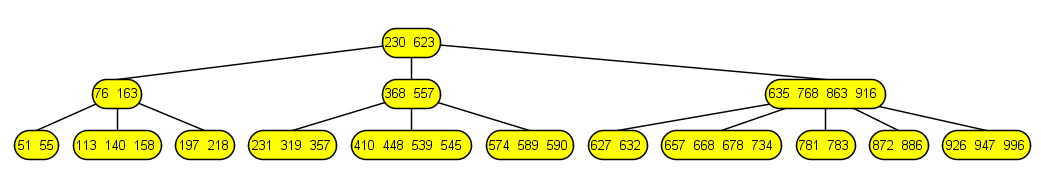
\includegraphics[width=1\textwidth]{Images/(a,b)-Tree/(3,5)-Tree_Search.png}
    \caption{(3,5)-Tree~\cite{gnarley_trees}}
    \label{fig:a_b_tree:a_b_tree_example}
  \end{figure}
\end{frame}

%-------------------------------------------------------------------------------

\begin{frame}{(a,b)-Trees}{Implementation - Insert}
  \textbf{Inserting an element:} (\texttt{\color{MainA}insert})
  \begin{itemize}
    \item<2->
      Search the position to insert the key into
    \item<3->
      This position will always be an leaf
    \item<4->
      Insert the element into the tree
    \item<5->
      \textbf{Attention:} As a result node can overflow by one element\\
      (Degree {\color{MainA}$b+1$})
    \item<6-> Then we \textbf{split} the node
  \end{itemize}
\end{frame}

%-------------------------------------------------------------------------------

\begin{frame}{(a,b)-Trees}{Implementation - Insert}
  \textbf{Inserting an element:} (\texttt{\color{MainA}insert})
    \begin{figure}
    \begin{columns}
      \begin{column}{0.35\linewidth}
        \begin{adjustbox}{width=\linewidth}
          \begin{tikzpicture}[
  node/.style={
    rectangle,
    color=black,
    draw=Mittel-Blau,
    fill=Hell-Blau,
    line width=0.15em,
    minimum size=2.0em,
    inner sep=0em
  }, path_start/.style={
%    -{Computer Modern Rightarrow[length=0.5em]},
    -{Stealth[length=1.25em]},
    line width=0.25em,
    color=Mittel-Gruen
  }, path/.style={
    path_start,
%    {Circle[scale=0.5,round]}-{Computer Modern Rightarrow[length=0.5em]},
    {Circle[scale=0.5,round]}-{Stealth[length=1.25em]},
    shorten <=-0.35em
  }, level/.style={
    sibling distance=0.0em,
    level distance=5.0em
  }, background/.style={
    fill=black!20!white,
    color=black!20!white
  }, full/.style={
    fill=orange!40!yellow,
    draw=red!20!orange
  }]
\node [node, xshift=-1em, background] { }
child [path, -, xshift=-5em, yshift=2em, background, edge from parent path={
  (\tikzparentnode.south west) -- (\tikzchildnode.north)}
] { };
\node [node, xshift=1em, background] { }
child [path, xshift=-1em, edge from parent path={
  (\tikzparentnode.south west) -- (node1.north east)}
] {
  node [node, full, xshift=-3em] {2}
  node [node, full, xshift=-1em] (node1) {10}
  node [node, full, xshift=1em] {15}
  node [node, full, xshift=3em] {24}
}
child [path, -, xshift=5em, yshift=2em, background, edge from parent path={
  (\tikzparentnode.south east) -- (\tikzchildnode.north)}
] { };
\end{tikzpicture}
        \end{adjustbox}
      \end{column}
      \begin{column}{0.1\linewidth}
        \begin{center}
          $\Rightarrow$
        \end{center}
      \end{column}
      \begin{column}{0.35\linewidth}
        \begin{adjustbox}{width=\linewidth}
          \begin{tikzpicture}[
  node/.style={
    rectangle,
    color=black,
    draw=Mittel-Blau,
    fill=Hell-Blau,
    line width=0.15em,
    minimum size=2.0em,
    inner sep=0em
  }, path_start/.style={
%    -{Computer Modern Rightarrow[length=0.5em]},
    -{Stealth[length=1.25em]},
    line width=0.25em,
    color=Mittel-Gruen
  }, path/.style={
    path_start,
%    {Circle[scale=0.5,round]}-{Computer Modern Rightarrow[length=0.5em]},
    {Circle[scale=0.5,round]}-{Stealth[length=1.25em]},
    shorten <=-0.35em
  }, level/.style={
    sibling distance=0.0em,
    level distance=5.0em
  }, background/.style={
    fill=black!20!white,
    color=black!20!white
  }, full/.style={
    fill=orange!40!yellow,
    draw=orange
  }]
\node [node, xshift=-2em, background] { }
child [path, -, xshift=-5em, yshift=2em, background, edge from parent path={
  (\tikzparentnode.south west) -- (\tikzchildnode.north)}
] { };
\node [node, xshift=2em, background] { }
child [path, -, xshift=5em, yshift=2em, background, edge from parent path={
  (\tikzparentnode.south east) -- (\tikzchildnode.north)}
] { };
\node [node] {15}
child [path, xshift=-2em, edge from parent path={
  (\tikzparentnode.south west) -- (node1.north east)}
] {
  node [node, xshift=-1em] (node1) {2}
  node [node, xshift=1em] {10}
}
child [path, xshift=1em, edge from parent path={
  (\tikzparentnode.south east) -- (\tikzchildnode.north)}
] {
  node [node, xshift=1em] {24}
};
\end{tikzpicture}
        \end{adjustbox}
      \end{column}
    \end{columns}
    \caption{Splitting a node}
    \label{fig:a_b_tree:insert_node_split}
    \end{figure}
    \vspace{-1.0em}
  \begin{itemize}
    \item<2->
      If the degree is higher than {\color{MainA}$b+1$}
      we split the node
    \item<3->
      This results in a node with
      {\color{MainA}$\mathrm{ceil}\left(\frac{b-1}{2}\right)$} elements,
      a node with
      {\color{MainA}$\mathrm{floor}\left(\frac{b-1}{2}\right)$} elements
      and one element for the parent node
    \item<4->
      Thats why we have the limit {\color{MainA}$b \geq 2\,a - 1$}
  \end{itemize}
\end{frame}

%-------------------------------------------------------------------------------

\begin{frame}{(a,b)-Trees}{Implementation - Insert}
  \textbf{Inserting an element:} (\texttt{\color{MainA}insert})
  \begin{itemize}
    \item<2->
      If the degree is higher than {\color{MainA}$b+1$}
      we split the node
    \item<3->
      Now the parent node can be of a higher degree than
      {\color{MainA}$b+1$}
    \item<4->
      We {\color{MainA}split} the parent nodes the same way
    \item<5->
      If we split the root node we create a new parent root node\\
      (The tree is now one level deeper)
  \end{itemize}
\end{frame}

%-------------------------------------------------------------------------------

\begin{frame}{(a,b)-Trees}{Implementation - Remove}
  \textbf{Removing an element:} (\texttt{\color{MainA}remove})
  \begin{itemize}
    \item<2->
      Search the element in {\color{MainA}$O(\log n)$} time
    \item<3->
      \textbf{Case 1:}
      The element is contained by a leaf
      \begin{itemize}
        \item Remove element
      \end{itemize}
    \item<4->
      \textbf{Case 2:}
      The element is contained by an inner node
      \begin{itemize}
        \item<5->
          Search the {\color{MainA}successor} in the right subtree
        \item<6->
          The {\color{MainA}successor} is always contained by a leaf
        \item<7->
          Replace the element with its {\color{MainA}successor} and
          delete the {\color{MainA}successor} from the leaf
      \end{itemize}
    \item<8->
      \textbf{Attention:}
      The leaf might be too small (degree of {\color{MainA}$a-1$})\\
      $\Rightarrow$ We {\color{MainA}rebalance} the tree
  \end{itemize}
\end{frame}

%-------------------------------------------------------------------------------

\begin{frame}{(a,b)-Trees}{Implementation - Remove}
  \textbf{Removing an element:} (\texttt{\color{MainA}remove})
  \begin{itemize}
    \item<2->
      \textbf{Attention:} The leaf might be too small
      (degree of {\color{MainA}$a-1$})\\
      $\Rightarrow$ We {\color{MainA}rebalance} the tree
      \vspace{0.5em}
      \begin{itemize}
        \item<3->
        \textbf{Case a:}
        If the left or right neighbour node has a degree
        {\color{MainA}greater than a} we \textbf{borrow} one element
        from this node
      \end{itemize}
      \onslide<4->
      \begin{figure}
        \begin{columns}
          \begin{column}{0.45\linewidth}
            \begin{adjustbox}{width=\linewidth}
              \begin{tikzpicture}[
  node/.style={
    rectangle,
    color=black,
    draw=Mittel-Blau,
    fill=Hell-Blau,
    line width=0.15em,
    minimum size=2.0em,
    inner sep=0em
  }, path_start/.style={
%    -{Computer Modern Rightarrow[length=0.5em]},
    -{Stealth[length=1.25em]},
    line width=0.25em,
    color=Mittel-Gruen
  }, path/.style={
    path_start,
%    {Circle[scale=0.5,round]}-{Computer Modern Rightarrow[length=0.5em]},
    {Circle[scale=0.5,round]}-{Stealth[length=1.25em]},
    shorten <=-0.35em
  }, level/.style={
    sibling distance=0.0em,
    level distance=5.0em
  }, background/.style={
    fill=black!20!white,
    color=black!20!white
  }, full/.style={
    fill=orange!40!yellow,
    draw=orange
  }]
\node [node, xshift=-2em, background] { }
child [path, -, xshift=-5em, yshift=2em, background, edge from parent path={
  (\tikzparentnode.south west) -- (\tikzchildnode.north)}
] { };
\node [node, xshift=2em, background] { }
child [path, -, xshift=5em, yshift=2em, background, edge from parent path={
  (\tikzparentnode.south east) -- (\tikzchildnode.north)}
] { };
\node [node] {15}
child [path, xshift=-2em, edge from parent path={
  (\tikzparentnode.south west) -- (node1.north)}
] {
  node [node, xshift=-2em] {2}
  node [node, xshift=0em] (node1) {7}
  node [node, xshift=2em] {10}
}
child [path, xshift=2em, edge from parent path={
  (\tikzparentnode.south east) -- (\tikzchildnode.north)}
] {
  node [node, xshift=1em, minimum width=0.5em] {}
};
\end{tikzpicture}

            \end{adjustbox}
          \end{column}
          \begin{column}{0.1\linewidth}
            \begin{center}
              $\Rightarrow$
            \end{center}
          \end{column}
          \begin{column}{0.45\linewidth}
            \begin{adjustbox}{width=\linewidth}
              \begin{tikzpicture}[
  node/.style={
    rectangle,
    color=black,
    draw=Mittel-Blau,
    fill=Hell-Blau,
    line width=0.15em,
    minimum size=2.0em,
    inner sep=0em
  }, path_start/.style={
%    -{Computer Modern Rightarrow[length=0.5em]},
    -{Stealth[length=1.25em]},
    line width=0.25em,
    color=Mittel-Gruen
  }, path/.style={
    path_start,
%    {Circle[scale=0.5,round]}-{Computer Modern Rightarrow[length=0.5em]},
    {Circle[scale=0.5,round]}-{Stealth[length=1.25em]},
    shorten <=-0.35em
  }, level/.style={
    sibling distance=0.0em,
    level distance=5.0em
  }, background/.style={
    fill=black!20!white,
    color=black!20!white
  }, full/.style={
    fill=orange!40!yellow,
    draw=orange
  }]
\node [node, xshift=-2em, background] { }
child [path, -, xshift=-5em, yshift=2em, background, edge from parent path={
  (\tikzparentnode.south west) -- (\tikzchildnode.north)}
] { };
\node [node, xshift=2em, background] { }
child [path, -, xshift=5em, yshift=2em, background, edge from parent path={
  (\tikzparentnode.south east) -- (\tikzchildnode.north)}
] { };
\node [node] {10}
child [path, xshift=-2em, edge from parent path={
  (\tikzparentnode.south west) -- (node1.north east)}
] {
  node [node, xshift=-1em] (node1) {2}
  node [node, xshift=1em] {7}
}
child [path, xshift=2em, edge from parent path={
  (\tikzparentnode.south east) -- (\tikzchildnode.north)}
] {
  node [node] {15}
};
\end{tikzpicture}
            \end{adjustbox}
          \end{column}
        \end{columns}
        \caption{Borrow an element}
        \label{fig:a_b_tree:move}
      \end{figure}
  \end{itemize}
\end{frame}

%-------------------------------------------------------------------------------

\begin{frame}{(a,b)-Trees}{Implementation - Remove}
  \textbf{Removing an element:} (\texttt{\color{MainA}remove})
  \begin{itemize}
    \item<2->
      \textbf{Attention:} The leaf might be too small (degree of {\color{MainA}$a-1$})\\
      $\Rightarrow$ We {\color{MainA}rebalance} the tree
      \vspace{0.5em}
      \begin{itemize}
        \item<3->
          \textbf{Case b:}
          We {\color{MainA}merge} the node with its right or left
          neighbour
      \end{itemize}
      \onslide<4->
      \begin{figure}
        \begin{columns}
          \begin{column}{0.45\linewidth}
            \begin{adjustbox}{width=\linewidth}
              \begin{tikzpicture}[
  node/.style={
    rectangle,
    color=black,
    draw=Mittel-Blau,
    fill=Hell-Blau,
    line width=0.15em,
    minimum size=2.0em,
    inner sep=0em
  }, path_start/.style={
%    -{Computer Modern Rightarrow[length=0.5em]},
    -{Stealth[length=1.25em]},
    line width=0.25em,
    color=Mittel-Gruen
  }, path/.style={
    path_start,
%    {Circle[scale=0.5,round]}-{Computer Modern Rightarrow[length=0.5em]},
    {Circle[scale=0.5,round]}-{Stealth[length=1.25em]},
    shorten <=-0.35em
  }, level/.style={
    sibling distance=0.0em,
    level distance=5.0em
  }, background/.style={
    fill=black!20!white,
    color=black!20!white
  }, full/.style={
    fill=orange!40!yellow,
    draw=orange
  }]
\node [node, xshift=-2em, background] { }
child [path, -, xshift=-5em, yshift=2em, background, edge from parent path={
  (\tikzparentnode.south west) -- (\tikzchildnode.north)}
] { };
\node [node, xshift=2em, background] { }
child [path, -, xshift=5em, yshift=2em, background, edge from parent path={
  (\tikzparentnode.south east) -- (\tikzchildnode.north)}
] { };
\node [node] {23}
child [path, xshift=-2em, edge from parent path={
  (\tikzparentnode.south west) -- (\tikzchildnode.north)}
] {
  node [node] {17}
}
child [path, xshift=2em, edge from parent path={
  (\tikzparentnode.south east) -- (\tikzchildnode.north)}
] {
  node [node, xshift=1em, minimum width=0.5em] {}
};
\end{tikzpicture}
            \end{adjustbox}
          \end{column}
          \begin{column}{0.1\linewidth}
            \begin{center}
              $\Rightarrow$
            \end{center}
          \end{column}
          \begin{column}{0.45\linewidth}
            \begin{adjustbox}{width=0.85\linewidth}
              \begin{tikzpicture}[
  node/.style={
    rectangle,
    color=black,
    draw=Mittel-Blau,
    fill=Hell-Blau,
    line width=0.15em,
    minimum size=2.0em,
    inner sep=0em
  }, path_start/.style={
%    -{Computer Modern Rightarrow[length=0.5em]},
    -{Stealth[length=1.25em]},
    line width=0.25em,
    color=Mittel-Gruen
  }, path/.style={
    path_start,
%    {Circle[scale=0.5,round]}-{Computer Modern Rightarrow[length=0.5em]},
    {Circle[scale=0.5,round]}-{Stealth[length=1.25em]},
    shorten <=-0.35em
  }, level/.style={
    sibling distance=0.0em,
    level distance=5.0em
  }, background/.style={
    fill=black!20!white,
    color=black!20!white
  }, full/.style={
    fill=orange!40!yellow,
    draw=red!20!orange
  }]
\node [node, xshift=-1em, background] { }
child [path, -, xshift=-5em, yshift=2em, background, edge from parent path={
  (\tikzparentnode.south west) -- (\tikzchildnode.north)}
] { };
\node [node, xshift=1em, background] { }
child [path, xshift=-1em, edge from parent path={
  (\tikzparentnode.south west) -- (node1.north east)}
] {
  node [node, xshift=-1em] (node1) {17}
  node [node, xshift=1em] {23}
}
child [path, -, xshift=5em, yshift=2em, background, edge from parent path={
  (\tikzparentnode.south east) -- (\tikzchildnode.north)}
] { };
\end{tikzpicture}
            \end{adjustbox}
          \end{column}
        \end{columns}
        \caption{Merge two nodes}
        \label{fig:a_b_tree:merge}
      \end{figure}
  \end{itemize}
\end{frame}

%-------------------------------------------------------------------------------

\begin{frame}{(a,b)-Trees}{Implementation - Remove}
  \textbf{Removing an element:} (\texttt{\color{MainA}remove})
  \begin{itemize}
    \item<2->
      Now the parent node can be of degree {\color{MainA}$a-1$}
    \item<3->
      We {\color{MainA}merge} parent nodes the same way
    \item<4->
      If the root has only a single child
      \begin{itemize}
        \item
          Remove the root
        \item
          Define sole child as new root
        \item
          The tree shrinks by one level
      \end{itemize}
  \end{itemize}
\end{frame}

%-------------------------------------------------------------------------------

\subsubsection{Runtime Complexity}

\begin{frame}{(a,b)-Trees}{Runtime Complexity}
  \textbf{Runtime complexity of \texttt{\color{MainA}lookup},
    \texttt{\color{MainA}insert} and \texttt{\color{MainA}remove}:}
  \begin{itemize}
    \item<2->
      All operations in {\color{MainA}$O(d)$} with
      {\color{MainA}$d$} being the depth of the tree
    \item<3->
      Each node (except the root) has {\color{MainA}more than $a$
      children}\\
      \begin{math}
        \Rightarrow
        \color{MainA}
        n \geq a^{d-1}
      \end{math}
      and
      \begin{math}
        \color{MainA}
        d \leq 1 + \log_a n = O(log_a n)
      \end{math}
  \end{itemize}
  \vspace{1em}
  \onslide<4->\textbf{In detail:}
  \begin{itemize}
    \item<5->
      \texttt{\color{MainA}lookup} always takes $\color{MainA}\Theta(d)$
    \item<6->
      \texttt{\color{MainA}insert} and
      \texttt{\color{MainA}remove}
      often require only {\color{MainA}$O(1)$} time
    \item<7->
      \textbf{Worst case:} {\color{MainA}split} or
      {\color{MainA}merge} all nodes on path up to the root
    \item<8->
      Therefore instead of {\color{MainA}$b \geq 2 \, a - 1$}
      we need {\color{MainA}$b \geq 2 \, a$}
  \end{itemize}
\end{frame}

%-------------------------------------------------------------------------------

%% \begin{frame}{(a,b)-Trees}{Runtime Complexity}
%%   \textbf{Runtime complexity of \texttt{\color{MainA}lookup},
%%     \texttt{\color{MainA}insert} and \texttt{\color{MainA}remove}:}
%%   \begin{itemize}
%%     \item<2->
%%       If we look closer:
%%       \begin{itemize}
%%         \item<3->
%%           \texttt{\color{MainA}insert} and
%%           \texttt{\color{MainA}remove}
%%           often require only {\color{MainA}$O(1)$} time
%%         \item<4->
%%           Only in the {\color{MainA}worst case} we have to
%%           {\color{MainA}split} or
%%           {\color{MainA}combine} all nodes on a path up to the root
%%       \end{itemize}
%%     \item<5->
%%       We need {\color{MainA}$b \geq 2 \, a$} instead of
%%       {\color{MainA}$b \geq 2 \, a - 1$}
%%     \item<6->
%%       Here is a negative example of a (2,3)-tree
%%   \end{itemize}
%% \end{frame}

%-------------------------------------------------------------------------------

\begin{frame}{(a,b)-Trees}{Runtime Complexity - Counter-example for (2,3)-Tree}
  \textbf{Counter example (2,3)-Tree:}
  \begin{itemize}
    \item<2->
      Before executing \texttt{\color{MainA}delete(11)}
   \onslide<3->
  \end{itemize}
  \begin{figure}
    \begin{adjustbox}{width=0.6\linewidth}
      \begin{tikzpicture}[
  node/.style={
    rectangle,
    color=black,
    draw=Mittel-Blau,
    fill=Hell-Blau,
    line width=0.15em,
    minimum size=2.0em,
    inner sep=0em
  }, path_start/.style={
%    -{Computer Modern Rightarrow[length=0.5em]},
    -{Stealth[length=1.25em]},
    line width=0.25em,
    color=Mittel-Gruen
  }, path/.style={
    path_start,
%    {Circle[scale=0.5,round]}-{Computer Modern Rightarrow[length=0.5em]},
    {Circle[scale=0.5,round]}-{Stealth[length=1.25em]},
    shorten <=-0.35em
  }, level/.style={
    sibling distance=0.0em,
    level distance=5.0em
  }]
\node [node] {8}
child [path, xshift=-6em, edge from parent path={
  (\tikzparentnode.south west) -- (\tikzchildnode.north)}
] {
  node [node, xshift=0em] {4}
  child [path, xshift=-3.0em, edge from parent path={
    (\tikzparentnode.south west) -- (\tikzchildnode.north)}
  ] {
    node [node] {2}
    child [path, xshift=-1.5em, edge from parent path={
      (\tikzparentnode.south west) -- (\tikzchildnode.north)}
    ] { node [node] {1} }
    child [path, xshift=1.5em, edge from parent path={
      (\tikzparentnode.south east) -- (\tikzchildnode.north)}
    ] { node [node] {3} }
  }
  child [path, xshift=3.0em, edge from parent path={
    (\tikzparentnode.south east) -- (\tikzchildnode.north)}
  ] {
    node [node] {6}
    child [path, xshift=-1.5em, edge from parent path={
      (\tikzparentnode.south west) -- (\tikzchildnode.north)}
    ] { node [node] {5} }
    child [path, xshift=1.5em, edge from parent path={
      (\tikzparentnode.south east) -- (\tikzchildnode.north)}
    ] { node [node] {7} }
  }
}
child [path, xshift=6em, edge from parent path={
  (\tikzparentnode.south east) -- (\tikzchildnode.north)}
] {
  node [node, xshift=0em] {12}
  child [path, xshift=-3.0em, edge from parent path={
    (\tikzparentnode.south west) -- (\tikzchildnode.north)}
  ] {
    node [node] {10}
    child [path, xshift=-1.5em, edge from parent path={
      (\tikzparentnode.south west) -- (\tikzchildnode.north)}
    ] { node [node] {9} }
    child [path, xshift=1.5em, edge from parent path={
      (\tikzparentnode.south east) -- (\tikzchildnode.north)}
    ] { node [node] {11} }
  }
  child [path, xshift=3.0em, edge from parent path={
    (\tikzparentnode.south east) -- (\tikzchildnode.north)}
  ] {
    node [node] {14}
    child [path, xshift=-1.5em, edge from parent path={
      (\tikzparentnode.south west) -- (\tikzchildnode.north)}
    ] { node [node] {13} }
    child [path, xshift=1.5em, edge from parent path={
      (\tikzparentnode.south east) -- (\tikzchildnode.north)}
    ] { node [node] {15} }
  }
};
\end{tikzpicture}
    \end{adjustbox}
    \label{fig:a_b_tree:2_3_tree_1}
    \caption{Normal (2,3)-Tree}
  \end{figure}
\end{frame}

%-------------------------------------------------------------------------------

\begin{frame}{(a,b)-Trees}{Runtime Complexity - Counter example for (2,3)-Tree}
  \textbf{Counter example (2,3)-Tree:}
  \begin{itemize}
  \item
    Executing \texttt{\color{MainA}delete(11)}
  \end{itemize}
  \begin{figure}
    \begin{adjustbox}{width=0.6\linewidth}
      \begin{tikzpicture}[
  node/.style={
    rectangle,
    color=black,
    draw=Mittel-Blau,
    fill=Hell-Blau,
    line width=0.15em,
    minimum size=2.0em,
    inner sep=0em
  }, path_start/.style={
%    -{Computer Modern Rightarrow[length=0.5em]},
    -{Stealth[length=1.25em]},
    line width=0.25em,
    color=Mittel-Gruen
  }, path/.style={
    path_start,
%    {Circle[scale=0.5,round]}-{Computer Modern Rightarrow[length=0.5em]},
    {Circle[scale=0.5,round]}-{Stealth[length=1.25em]},
    shorten <=-0.35em
  }, level/.style={
    sibling distance=0.0em,
    level distance=5.0em
  }]
\node [node] {8}
child [path, xshift=-6em, edge from parent path={
  (\tikzparentnode.south west) -- (\tikzchildnode.north)}
] {
  node [node, xshift=0em] {4}
  child [path, xshift=-3.0em, edge from parent path={
    (\tikzparentnode.south west) -- (\tikzchildnode.north)}
  ] {
    node [node] {2}
    child [path, xshift=-1.5em, edge from parent path={
      (\tikzparentnode.south west) -- (\tikzchildnode.north)}
    ] { node [node] {1} }
    child [path, xshift=1.5em, edge from parent path={
      (\tikzparentnode.south east) -- (\tikzchildnode.north)}
    ] { node [node] {3} }
  }
  child [path, xshift=3.0em, edge from parent path={
    (\tikzparentnode.south east) -- (\tikzchildnode.north)}
  ] {
    node [node] {6}
    child [path, xshift=-1.5em, edge from parent path={
      (\tikzparentnode.south west) -- (\tikzchildnode.north)}
    ] { node [node] {5} }
    child [path, xshift=1.5em, edge from parent path={
      (\tikzparentnode.south east) -- (\tikzchildnode.north)}
    ] { node [node] {7} }
  }
}
child [path, xshift=6em, edge from parent path={
  (\tikzparentnode.south east) -- (\tikzchildnode.north)}
] {
  node [node, xshift=0em] {12}
  child [path, xshift=-3.0em, edge from parent path={
    (\tikzparentnode.south west) -- (\tikzchildnode.north)}
  ] {
    node [node] {10}
    child [path, xshift=-1.5em, edge from parent path={
      (\tikzparentnode.south west) -- (\tikzchildnode.north)}
    ] { node [node] {9} }
    child [path, xshift=1.5em, edge from parent path={
      (\tikzparentnode.south east) -- (\tikzchildnode.north)}
    ] { node [node, minimum width=0.5em] {} }
  }
  child [path, xshift=3.0em, edge from parent path={
    (\tikzparentnode.south east) -- (\tikzchildnode.north)}
  ] {
    node [node] {14}
    child [path, xshift=-1.5em, edge from parent path={
      (\tikzparentnode.south west) -- (\tikzchildnode.north)}
    ] { node [node] {13} }
    child [path, xshift=1.5em, edge from parent path={
      (\tikzparentnode.south east) -- (\tikzchildnode.north)}
    ] { node [node] {15} }
  }
};
\end{tikzpicture}
    \end{adjustbox}
    \label{fig:a_b_tree:2_3_tree_2}
    \caption{(2,3)-Tree - Delete step 1}
  \end{figure}
\end{frame}

%-------------------------------------------------------------------------------

\begin{frame}{(a,b)-Trees}{Runtime Complexity - Counter example for (2,3)-Tree}
  \textbf{Counter example (2,3)-Tree:}
  \begin{itemize}
    \item
      Executing \texttt{\color{MainA}delete(11)}
  \end{itemize}
  \begin{figure}
    \begin{adjustbox}{width=0.6\linewidth}
      \begin{tikzpicture}[
  node/.style={
    rectangle,
    color=black,
    draw=Mittel-Blau,
    fill=Hell-Blau,
    line width=0.15em,
    minimum size=2.0em,
    inner sep=0em
  }, path_start/.style={
%    -{Computer Modern Rightarrow[length=0.5em]},
    -{Stealth[length=1.25em]},
    line width=0.25em,
    color=Mittel-Gruen
  }, path/.style={
    path_start,
%    {Circle[scale=0.5,round]}-{Computer Modern Rightarrow[length=0.5em]},
    {Circle[scale=0.5,round]}-{Stealth[length=1.25em]},
    shorten <=-0.35em
  }, level/.style={
    sibling distance=0.0em,
    level distance=5.0em
  }]
\node [node] {8}
child [path, xshift=-6em, edge from parent path={
  (\tikzparentnode.south west) -- (\tikzchildnode.north)}
] {
  node [node, xshift=0em] {4}
  child [path, xshift=-3.0em, edge from parent path={
    (\tikzparentnode.south west) -- (\tikzchildnode.north)}
  ] {
    node [node] {2}
    child [path, xshift=-1.5em, edge from parent path={
      (\tikzparentnode.south west) -- (\tikzchildnode.north)}
    ] { node [node] {1} }
    child [path, xshift=1.5em, edge from parent path={
      (\tikzparentnode.south east) -- (\tikzchildnode.north)}
    ] { node [node] {3} }
  }
  child [path, xshift=3.0em, edge from parent path={
    (\tikzparentnode.south east) -- (\tikzchildnode.north)}
  ] {
    node [node] {6}
    child [path, xshift=-1.5em, edge from parent path={
      (\tikzparentnode.south west) -- (\tikzchildnode.north)}
    ] { node [node] {5} }
    child [path, xshift=1.5em, edge from parent path={
      (\tikzparentnode.south east) -- (\tikzchildnode.north)}
    ] { node [node] {7} }
  }
}
child [path, xshift=6em, edge from parent path={
  (\tikzparentnode.south east) -- (\tikzchildnode.north)}
] {
  node [node, xshift=0em] {12}
  child [path, xshift=-3.0em, edge from parent path={
    (\tikzparentnode.south west) -- (\tikzchildnode.north)}
  ] {
    node [node, minimum width=0.5em] {}
    child [path, edge from parent path={
      (\tikzparentnode.south west) -- (node1.north east)}
    ] {
      node [node, xshift=-1.0em] (node1) {9}
      node [node, xshift=1.0em] {10}
    }
  }
  child [path, xshift=3.0em, edge from parent path={
    (\tikzparentnode.south east) -- (\tikzchildnode.north)}
  ] {
    node [node] {14}
    child [path, xshift=-1.5em, edge from parent path={
      (\tikzparentnode.south west) -- (\tikzchildnode.north)}
    ] { node [node] {13} }
    child [path, xshift=1.5em, edge from parent path={
      (\tikzparentnode.south east) -- (\tikzchildnode.north)}
    ] { node [node] {15} }
  }
};
\end{tikzpicture}
    \end{adjustbox}
    \label{fig:a_b_tree:2_3_tree_3}
    \caption{(2,3)-Tree - Delete step 2}
  \end{figure}
\end{frame}

%-------------------------------------------------------------------------------

\begin{frame}{(a,b)-Trees}{Runtime Complexity - Counter example for (2,3)-Tree}
  \textbf{Counter example (2,3)-Tree:}
  \begin{itemize}
    \item
      Executing \texttt{\color{MainA}delete(11)}
  \end{itemize}
  \begin{figure}
    \begin{adjustbox}{width=0.6\linewidth}
      \begin{tikzpicture}[
  node/.style={
    rectangle,
    color=black,
    draw=Mittel-Blau,
    fill=Hell-Blau,
    line width=0.15em,
    minimum size=2.0em,
    inner sep=0em
  }, path_start/.style={
%    -{Computer Modern Rightarrow[length=0.5em]},
    -{Stealth[length=1.25em]},
    line width=0.25em,
    color=Mittel-Gruen
  }, path/.style={
    path_start,
%    {Circle[scale=0.5,round]}-{Computer Modern Rightarrow[length=0.5em]},
    {Circle[scale=0.5,round]}-{Stealth[length=1.25em]},
    shorten <=-0.35em
  }, level/.style={
    sibling distance=0.0em,
    level distance=5.0em
  }]
\node [node] {8}
child [path, xshift=-6em, edge from parent path={
  (\tikzparentnode.south west) -- (\tikzchildnode.north)}
] {
  node [node, xshift=0em] {4}
  child [path, xshift=-3.0em, edge from parent path={
    (\tikzparentnode.south west) -- (\tikzchildnode.north)}
  ] {
    node [node] {2}
    child [path, xshift=-1.5em, edge from parent path={
      (\tikzparentnode.south west) -- (\tikzchildnode.north)}
    ] { node [node] {1} }
    child [path, xshift=1.5em, edge from parent path={
      (\tikzparentnode.south east) -- (\tikzchildnode.north)}
    ] { node [node] {3} }
  }
  child [path, xshift=3.0em, edge from parent path={
    (\tikzparentnode.south east) -- (\tikzchildnode.north)}
  ] {
    node [node] {6}
    child [path, xshift=-1.5em, edge from parent path={
      (\tikzparentnode.south west) -- (\tikzchildnode.north)}
    ] { node [node] {5} }
    child [path, xshift=1.5em, edge from parent path={
      (\tikzparentnode.south east) -- (\tikzchildnode.north)}
    ] { node [node] {7} }
  }
}
child [path, xshift=6em, edge from parent path={
  (\tikzparentnode.south east) -- (\tikzchildnode.north)}
] {
  node [node, minimum width=0.5em] {}
  child [path, edge from parent path={
    (\tikzparentnode.south west) -- (node2.north east)}
  ] {
    node [node, xshift=-1.0em] (node2) {12}
    child [path, xshift=-2.5em, edge from parent path={
      (\tikzparentnode.south west) -- (node1.north east)}
    ] {
      node [node, xshift=-1.0em] (node1) {9}
      node [node, xshift=1.0em] {10}
    }
    node [node, xshift=1.0em] {14}
    child [path, xshift=-0.5em, edge from parent path={
      (\tikzparentnode.south west) -- (\tikzchildnode.north)}
    ] { node [node] {13} }
    child [path, xshift=2.5em, edge from parent path={
      (\tikzparentnode.south east) -- (\tikzchildnode.north)}
    ] { node [node] {15} }
  }
};
\end{tikzpicture}
    \end{adjustbox}
    \label{fig:a_b_tree:2_3_tree_4}
    \caption{(2,3)-Tree - Delete step 3}
  \end{figure}
\end{frame}

%-------------------------------------------------------------------------------

\begin{frame}{(a,b)-Trees}{Runtime Complexity - Counter example for (2,3)-Tree}
  \textbf{Counter example (2,3)-Tree:}
  \begin{itemize}
    \item
      Executed \texttt{\color{MainA}delete(11)}
  \end{itemize}
  \begin{figure}
    \begin{adjustbox}{width=0.6\linewidth}
      \begin{tikzpicture}[
  node/.style={
    rectangle,
    color=black,
    draw=Mittel-Blau,
    fill=Hell-Blau,
    line width=0.15em,
    minimum size=2.0em,
    inner sep=0em
  }, path_start/.style={
%    -{Computer Modern Rightarrow[length=0.5em]},
    -{Stealth[length=1.25em]},
    line width=0.25em,
    color=Mittel-Gruen
  }, path/.style={
    path_start,
%    {Circle[scale=0.5,round]}-{Computer Modern Rightarrow[length=0.5em]},
    {Circle[scale=0.5,round]}-{Stealth[length=1.25em]},
    shorten <=-0.35em
  }, level/.style={
    sibling distance=0.0em,
    level distance=5.0em
  }]
\node [node, xshift=-1em] {4}
child [path, xshift=-7.0em, edge from parent path={
  (\tikzparentnode.south west) -- (\tikzchildnode.north)}
] {
  node [node] {2}
  child [path, xshift=-1.5em, edge from parent path={
    (\tikzparentnode.south west) -- (\tikzchildnode.north)}
  ] { node [node] {1} }
  child [path, xshift=1.5em, edge from parent path={
    (\tikzparentnode.south east) -- (\tikzchildnode.north)}
  ] { node [node] {3} }
}
node [node, xshift=1em] {8}
child [path, xshift=-3.0em, edge from parent path={
  (\tikzparentnode.south west) -- (\tikzchildnode.north)}
] {
  node [node] {6}
  child [path, xshift=-1.5em, edge from parent path={
    (\tikzparentnode.south west) -- (\tikzchildnode.north)}
  ] { node [node] {5} }
  child [path, xshift=1.5em, edge from parent path={
    (\tikzparentnode.south east) -- (\tikzchildnode.north)}
  ] { node [node] {7} }
}
child [path, xshift=6.0em, edge from parent path={
  (\tikzparentnode.south east) -- (node2.north east)}
] {
  node [node, xshift=-1.0em] (node2) {12}
  child [path, xshift=-2.5em, edge from parent path={
    (\tikzparentnode.south west) -- (node1.north east)}
  ] {
    node [node, xshift=-1.0em] (node1) {9}
    node [node, xshift=1.0em] {10}
  }
  node [node, xshift=1.0em] {14}
  child [path, xshift=-0.5em, edge from parent path={
    (\tikzparentnode.south west) -- (\tikzchildnode.north)}
  ] { node [node] {13} }
  child [path, xshift=2.5em, edge from parent path={
    (\tikzparentnode.south east) -- (\tikzchildnode.north)}
  ] { node [node] {15} }
};
\end{tikzpicture}
    \end{adjustbox}
    \label{fig:a_b_tree:2_3_tree_5}
    \caption{(2,3)-Tree - Delete step 4}
  \end{figure}
\end{frame}

%-------------------------------------------------------------------------------

\begin{frame}{(a,b)-Trees}{Runtime Complexity - Counter example for (2,3)-Tree}
  \textbf{Counter example (2,3)-Tree:}
  \begin{itemize}
    \item
      Executing \texttt{\color{MainA}insert(11)}
  \end{itemize}
  \onslide<3->
  \begin{figure}
    \begin{adjustbox}{width=0.7\linewidth}
      \begin{tikzpicture}[
  node/.style={
    rectangle,
    color=black,
    draw=Mittel-Blau,
    fill=Hell-Blau,
    line width=0.15em,
    minimum size=2.0em,
    inner sep=0em
  }, path_start/.style={
%    -{Computer Modern Rightarrow[length=0.5em]},
    -{Stealth[length=1.25em]},
    line width=0.25em,
    color=Mittel-Gruen
  }, path/.style={
    path_start,
%    {Circle[scale=0.5,round]}-{Computer Modern Rightarrow[length=0.5em]},
    {Circle[scale=0.5,round]}-{Stealth[length=1.25em]},
    shorten <=-0.35em
  }, level/.style={
    sibling distance=0.0em,
    level distance=5.0em
  }, full/.style={
    fill=orange!40!yellow,
    draw=orange
  }]
\node [node, xshift=-1em] {4}
child [path, xshift=-7.0em, edge from parent path={
  (\tikzparentnode.south west) -- (\tikzchildnode.north)}
] {
  node [node] {2}
  child [path, xshift=-1.5em, edge from parent path={
    (\tikzparentnode.south west) -- (\tikzchildnode.north)}
  ] { node [node] {1} }
  child [path, xshift=1.5em, edge from parent path={
    (\tikzparentnode.south east) -- (\tikzchildnode.north)}
  ] { node [node] {3} }
}
node [node, xshift=1em] {8}
child [path, xshift=-3.0em, edge from parent path={
  (\tikzparentnode.south west) -- (\tikzchildnode.north)}
] {
  node [node] {6}
  child [path, xshift=-1.5em, edge from parent path={
    (\tikzparentnode.south west) -- (\tikzchildnode.north)}
  ] { node [node] {5} }
  child [path, xshift=1.5em, edge from parent path={
    (\tikzparentnode.south east) -- (\tikzchildnode.north)}
  ] { node [node] {7} }
}
child [path, xshift=7.0em, edge from parent path={
  (\tikzparentnode.south east) -- (node2.north east)}
] {
  node [node, xshift=-1.0em] (node2) {12}
  child [path, xshift=-2.5em, edge from parent path={
    (\tikzparentnode.south west) -- (node1.north)}
  ] {
    node [node, full, xshift=-2.0em] {9}
    node [node, full, xshift=0.0em] (node1) {10}
    node [node, full, xshift=2.0em] {11}
  }
  node [node, xshift=1.0em] {14}
  child [path, xshift=0.5em, edge from parent path={
    (\tikzparentnode.south west) -- (\tikzchildnode.north)}
  ] { node [node] {13} }
  child [path, xshift=3.5em, edge from parent path={
    (\tikzparentnode.south east) -- (\tikzchildnode.north)}
  ] { node [node] {15} }
};
\end{tikzpicture}
    \end{adjustbox}
    \label{fig:a_b_tree:2_3_tree_6}
    \caption{(2,3)-Tree - Insert step 1}
  \end{figure}
\end{frame}

%-------------------------------------------------------------------------------

\begin{frame}{(a,b)-Trees}{Runtime Complexity - Counter example for (2,3)-Tree}
  \textbf{Counter example (2,3)-Tree:}
  \begin{itemize}
    \item
      Executing \texttt{\color{MainA}insert(11)}
  \end{itemize}
  \begin{figure}
    \begin{adjustbox}{width=0.7\linewidth}
      \begin{tikzpicture}[
  node/.style={
    rectangle,
    color=black,
    draw=Mittel-Blau,
    fill=Hell-Blau,
    line width=0.15em,
    minimum size=2.0em,
    inner sep=0em
  }, path_start/.style={
%    -{Computer Modern Rightarrow[length=0.5em]},
    -{Stealth[length=1.25em]},
    line width=0.25em,
    color=Mittel-Gruen
  }, path/.style={
    path_start,
%    {Circle[scale=0.5,round]}-{Computer Modern Rightarrow[length=0.5em]},
    {Circle[scale=0.5,round]}-{Stealth[length=1.25em]},
    shorten <=-0.35em
  }, level/.style={
    sibling distance=0.0em,
    level distance=5.0em
  }, full/.style={
    fill=orange!40!yellow,
    draw=orange
  }]
\node [node, xshift=-1em] {4}
child [path, xshift=-7.0em, edge from parent path={
  (\tikzparentnode.south west) -- (\tikzchildnode.north)}
] {
  node [node] {2}
  child [path, xshift=-1.5em, edge from parent path={
    (\tikzparentnode.south west) -- (\tikzchildnode.north)}
  ] { node [node] {1} }
  child [path, xshift=1.5em, edge from parent path={
    (\tikzparentnode.south east) -- (\tikzchildnode.north)}
  ] { node [node] {3} }
}
node [node, xshift=1em] {8}
child [path, xshift=-3.0em, edge from parent path={
  (\tikzparentnode.south west) -- (\tikzchildnode.north)}
] {
  node [node] {6}
  child [path, xshift=-1.5em, edge from parent path={
    (\tikzparentnode.south west) -- (\tikzchildnode.north)}
  ] { node [node] {5} }
  child [path, xshift=1.5em, edge from parent path={
    (\tikzparentnode.south east) -- (\tikzchildnode.north)}
  ] { node [node] {7} }
}
child [path, xshift=5.0em, edge from parent path={
  (\tikzparentnode.south east) -- (node2.north)}
] {
  node [node, full, xshift=-2.0em] {10}
  child [path, xshift=-1.5em, edge from parent path={
    (\tikzparentnode.south west) -- (\tikzchildnode.north)}
  ] { node [node] {9} }
  node [node, full, xshift=0.0em] (node2) {12}
  child [path, xshift=-0.5em, edge from parent path={
    (\tikzparentnode.south west) -- (\tikzchildnode.north)}
  ] { node [node] {11} }
  node [node, full, xshift=2.0em] {14}
  child [path, xshift=0.5em, edge from parent path={
    (\tikzparentnode.south west) -- (\tikzchildnode.north)}
  ] { node [node] {13} }
  child [path, xshift=3.5em, edge from parent path={
    (\tikzparentnode.south east) -- (\tikzchildnode.north)}
  ] { node [node] {15} }
};
\end{tikzpicture}
    \end{adjustbox}
    \label{fig:a_b_tree:2_3_tree_7}
    \caption{(2,3)-Tree - Insert step 2}
  \end{figure}
\end{frame}

%-------------------------------------------------------------------------------

\begin{frame}{(a,b)-Trees}{Runtime Complexity - Counter example for (2,3)-Tree}
  \textbf{Counter example (2,3)-Tree:}
  \begin{itemize}
    \item
      Executing \texttt{\color{MainA}insert(11)}
  \end{itemize}
  \begin{figure}
    \begin{adjustbox}{width=0.7\linewidth}
      \begin{tikzpicture}[
  node/.style={
    rectangle,
    color=black,
    draw=Mittel-Blau,
    fill=Hell-Blau,
    line width=0.15em,
    minimum size=2.0em,
    inner sep=0em
  }, path_start/.style={
%    -{Computer Modern Rightarrow[length=0.5em]},
    -{Stealth[length=1.25em]},
    line width=0.25em,
    color=Mittel-Gruen
  }, path/.style={
    path_start,
%    {Circle[scale=0.5,round]}-{Computer Modern Rightarrow[length=0.5em]},
    {Circle[scale=0.5,round]}-{Stealth[length=1.25em]},
    shorten <=-0.35em
  }, level/.style={
    sibling distance=0.0em,
    level distance=5.0em
  }, full/.style={
    fill=orange!40!yellow,
    draw=orange
  }]
\node [node, full, xshift=-2em] {4}
child [path, xshift=-7.0em, edge from parent path={
  (\tikzparentnode.south west) -- (\tikzchildnode.north)}
] {
  node [node] {2}
  child [path, xshift=-1.5em, edge from parent path={
    (\tikzparentnode.south west) -- (\tikzchildnode.north)}
  ] { node [node] {1} }
  child [path, xshift=1.5em, edge from parent path={
    (\tikzparentnode.south east) -- (\tikzchildnode.north)}
  ] { node [node] {3} }
}
node [node, full, xshift=0em] {8}
child [path, xshift=-3.0em, edge from parent path={
  (\tikzparentnode.south west) -- (\tikzchildnode.north)}
] {
  node [node] {6}
  child [path, xshift=-1.5em, edge from parent path={
    (\tikzparentnode.south west) -- (\tikzchildnode.north)}
  ] { node [node] {5} }
  child [path, xshift=1.5em, edge from parent path={
    (\tikzparentnode.south east) -- (\tikzchildnode.north)}
  ] { node [node] {7} }
}
node [node, full, xshift=2em] {12}
child [path, xshift=3.0em, edge from parent path={
  (\tikzparentnode.south west) -- (\tikzchildnode.north)}
] {
  node [node, xshift=-2.0em] {10}
  child [path, xshift=-1.5em, edge from parent path={
    (\tikzparentnode.south west) -- (\tikzchildnode.north)}
  ] { node [node] {9} }
  child [path, xshift=1.5em, edge from parent path={
    (\tikzparentnode.south east) -- (\tikzchildnode.north)}
  ] { node [node] {11} }
}
child [path, xshift=9.0em, edge from parent path={
  (\tikzparentnode.south east) -- (\tikzchildnode.north)}
] {
  node [node, xshift=-2.0em] {14}
  child [path, xshift=-1.5em, edge from parent path={
    (\tikzparentnode.south west) -- (\tikzchildnode.north)}
  ] { node [node] {13} }
  child [path, xshift=1.5em, edge from parent path={
    (\tikzparentnode.south east) -- (\tikzchildnode.north)}
  ] { node [node] {15} }
};
\end{tikzpicture}
    \end{adjustbox}
    \label{fig:a_b_tree:2_3_tree_8}
    \caption{(2,3)-Tree - Insert step 3}
  \end{figure}
\end{frame}

%-------------------------------------------------------------------------------

\begin{frame}{(a,b)-Trees}{Runtime Complexity - Counter example for (2,3)-Tree}
  \textbf{Counter example (2,3)-Tree:}
  \begin{itemize}
    \item
      Executed \texttt{\color{MainA}insert(11)}
  \end{itemize}
  \begin{figure}
    \begin{adjustbox}{width=0.6\linewidth}
      \begin{tikzpicture}[
  node/.style={
    rectangle,
    color=black,
    draw=Mittel-Blau,
    fill=Hell-Blau,
    line width=0.15em,
    minimum size=2.0em,
    inner sep=0em
  }, path_start/.style={
%    -{Computer Modern Rightarrow[length=0.5em]},
    -{Stealth[length=1.25em]},
    line width=0.25em,
    color=Mittel-Gruen
  }, path/.style={
    path_start,
%    {Circle[scale=0.5,round]}-{Computer Modern Rightarrow[length=0.5em]},
    {Circle[scale=0.5,round]}-{Stealth[length=1.25em]},
    shorten <=-0.35em
  }, level/.style={
    sibling distance=0.0em,
    level distance=5.0em
  }]
\node [node] {8}
child [path, xshift=-6em, edge from parent path={
  (\tikzparentnode.south west) -- (\tikzchildnode.north)}
] {
  node [node, xshift=0em] {4}
  child [path, xshift=-3.0em, edge from parent path={
    (\tikzparentnode.south west) -- (\tikzchildnode.north)}
  ] {
    node [node] {2}
    child [path, xshift=-1.5em, edge from parent path={
      (\tikzparentnode.south west) -- (\tikzchildnode.north)}
    ] { node [node] {1} }
    child [path, xshift=1.5em, edge from parent path={
      (\tikzparentnode.south east) -- (\tikzchildnode.north)}
    ] { node [node] {3} }
  }
  child [path, xshift=3.0em, edge from parent path={
    (\tikzparentnode.south east) -- (\tikzchildnode.north)}
  ] {
    node [node] {6}
    child [path, xshift=-1.5em, edge from parent path={
      (\tikzparentnode.south west) -- (\tikzchildnode.north)}
    ] { node [node] {5} }
    child [path, xshift=1.5em, edge from parent path={
      (\tikzparentnode.south east) -- (\tikzchildnode.north)}
    ] { node [node] {7} }
  }
}
child [path, xshift=6em, edge from parent path={
  (\tikzparentnode.south east) -- (\tikzchildnode.north)}
] {
  node [node, xshift=0em] {12}
  child [path, xshift=-3.0em, edge from parent path={
    (\tikzparentnode.south west) -- (\tikzchildnode.north)}
  ] {
    node [node] {10}
    child [path, xshift=-1.5em, edge from parent path={
      (\tikzparentnode.south west) -- (\tikzchildnode.north)}
    ] { node [node] {9} }
    child [path, xshift=1.5em, edge from parent path={
      (\tikzparentnode.south east) -- (\tikzchildnode.north)}
    ] { node [node] {11} }
  }
  child [path, xshift=3.0em, edge from parent path={
    (\tikzparentnode.south east) -- (\tikzchildnode.north)}
  ] {
    node [node] {14}
    child [path, xshift=-1.5em, edge from parent path={
      (\tikzparentnode.south west) -- (\tikzchildnode.north)}
    ] { node [node] {13} }
    child [path, xshift=1.5em, edge from parent path={
      (\tikzparentnode.south east) -- (\tikzchildnode.north)}
    ] { node [node] {15} }
  }
};
\end{tikzpicture}
    \end{adjustbox}
    \label{fig:a_b_tree:2_3_tree_9}
    \caption{(2,3)-Tree - Insert step 4}
  \end{figure}
\end{frame}

%-------------------------------------------------------------------------------

\begin{frame}{(a,b)-Trees}{Runtime Complexity - Counter example for (2,3)-Tree}
  \begin{columns}
    \begin{column}{0.6\linewidth}
      \textbf{Counter example (2,3)-Tree:}
      \begin{itemize}
        \item
          We are exactly where we started
        \item<2->
          If {\color{MainA}$b=2\,a-1$} then we can create a sequence of
          \texttt{\color{MainA}insert} and
          \texttt{\color{MainA}remove} operations where each operation
          costs {\color{MainA}$O(\log n)$}
        \item<3->
          We need {\color{MainA}$b \geq 2 \, a$} instead of
          {\color{MainA}$b \geq 2 \, a - 1$}
      \end{itemize}
    \end{column}
    \begin{column}{0.4\linewidth}
      \begin{figure}
        \begin{adjustbox}{width=\linewidth}
          \begin{tikzpicture}[
  node/.style={
    rectangle,
    color=black,
    draw=Mittel-Blau,
    fill=Hell-Blau,
    line width=0.15em,
    minimum size=2.0em,
    inner sep=0em
  }, path_start/.style={
%    -{Computer Modern Rightarrow[length=0.5em]},
    -{Stealth[length=1.25em]},
    line width=0.25em,
    color=Mittel-Gruen
  }, path/.style={
    path_start,
%    {Circle[scale=0.5,round]}-{Computer Modern Rightarrow[length=0.5em]},
    {Circle[scale=0.5,round]}-{Stealth[length=1.25em]},
    shorten <=-0.35em
  }, level/.style={
    sibling distance=0.0em,
    level distance=5.0em
  }]
\node [node] {8}
child [path, xshift=-6em, edge from parent path={
  (\tikzparentnode.south west) -- (\tikzchildnode.north)}
] {
  node [node, xshift=0em] {4}
  child [path, xshift=-3.0em, edge from parent path={
    (\tikzparentnode.south west) -- (\tikzchildnode.north)}
  ] {
    node [node] {2}
    child [path, xshift=-1.5em, edge from parent path={
      (\tikzparentnode.south west) -- (\tikzchildnode.north)}
    ] { node [node] {1} }
    child [path, xshift=1.5em, edge from parent path={
      (\tikzparentnode.south east) -- (\tikzchildnode.north)}
    ] { node [node] {3} }
  }
  child [path, xshift=3.0em, edge from parent path={
    (\tikzparentnode.south east) -- (\tikzchildnode.north)}
  ] {
    node [node] {6}
    child [path, xshift=-1.5em, edge from parent path={
      (\tikzparentnode.south west) -- (\tikzchildnode.north)}
    ] { node [node] {5} }
    child [path, xshift=1.5em, edge from parent path={
      (\tikzparentnode.south east) -- (\tikzchildnode.north)}
    ] { node [node] {7} }
  }
}
child [path, xshift=6em, edge from parent path={
  (\tikzparentnode.south east) -- (\tikzchildnode.north)}
] {
  node [node, xshift=0em] {12}
  child [path, xshift=-3.0em, edge from parent path={
    (\tikzparentnode.south west) -- (\tikzchildnode.north)}
  ] {
    node [node] {10}
    child [path, xshift=-1.5em, edge from parent path={
      (\tikzparentnode.south west) -- (\tikzchildnode.north)}
    ] { node [node] {9} }
    child [path, xshift=1.5em, edge from parent path={
      (\tikzparentnode.south east) -- (\tikzchildnode.north)}
    ] { node [node] {11} }
  }
  child [path, xshift=3.0em, edge from parent path={
    (\tikzparentnode.south east) -- (\tikzchildnode.north)}
  ] {
    node [node] {14}
    child [path, xshift=-1.5em, edge from parent path={
      (\tikzparentnode.south west) -- (\tikzchildnode.north)}
    ] { node [node] {13} }
    child [path, xshift=1.5em, edge from parent path={
      (\tikzparentnode.south east) -- (\tikzchildnode.north)}
    ] { node [node] {15} }
  }
};
\end{tikzpicture}
        \end{adjustbox}
        \vspace{-1.5em}
        \label{fig:a_b_tree:2_3_tree_10}
        \caption{(2,3)-Tree}
      \end{figure}
    \end{column}
  \end{columns}
\end{frame}

%-------------------------------------------------------------------------------

\begin{frame}{(a,b)-Trees}{Runtime Complexity - (2,4)-Tree}
  \textbf{(2,4)-Tree:}
  \begin{itemize}
    \item<2->
      If all nodes have {\color{MainA}2 children} we have to
      {\color{MainA}merge} the nodes up to the root on a
      \texttt{\color{MainA}remove} operation
    \item<3->
      If all nodes have {\color{MainA}4 children} we have to
      {\color{MainA}split} the nodes up to the root on a
      \texttt{\color{MainA}insert} operation
    \item<4->
      If all nodes have {\color{MainA}3 children} it takes some time
      to reach one of the previous two states
    \item<5->[$\Rightarrow$]
      \textbf{Nodes of degree 3 are stable}\\
      Neither an \texttt{\color{MainA}insert} nor a
      \texttt{\color{MainA}remove} operation trigger rebalancing
      operations
  \end{itemize}
\end{frame}

%-------------------------------------------------------------------------------

\begin{frame}{(a,b)-Trees}{Runtime Complexity - (2,4)-Tree}
  \textbf{(2,4)-Tree:}
  \begin{itemize}
    \item
      \textbf{Idea:}
      \begin{itemize}
        \item<2->
          After an expensive operation the tree is in a stable state
        \item<3->
          It takes some time until the next expensive operation occurs
      \end{itemize}
    \item<4->
      Like with dynamic arrays:
      \begin{itemize}
        \item<5->
          {\color{MainA}Reallocation} is expensive but it takes some time
          until the next expensive operation occurs
        \item<6->
          If we {\color{MainA}overallocate} clever we have an amortized
          runtime of {\color{MainA}$O(1)$}
      \end{itemize}
  \end{itemize}
\end{frame}

%-------------------------------------------------------------------------------

\begin{frame}{(a,b)-Trees}{Runtime Complexity - (2,4)-Tree}
  \textbf{Terminology:}
  \begin{itemize}
    \item<2->
      We analyze a sequence of {\color{MainA}$n$} operations
    \item<3->
      Let {\color{MainA}$\Phi_i$} be the potential of the tree after
      the {\color{MainA}$i$}-\textit{th} operation
    \item<4->
      {\color{MainA}$\Phi_i$}
      $=$ the number of stable nodes with {\color{MainA}degree 3}
    \item<5->
      Empty tree has 0 nodes: ${\color{MainA}\Phi} = 0$
  \end{itemize}
\end{frame}

%-------------------------------------------------------------------------------

\begin{frame}{(a,b)-Trees}{Runtime Complexity - (2,4)-Tree}
  \textbf{Example:}
  \begin{itemize}
    \item<2->
      Nodes of {\color{MainA}degree 3} are highlighted
  \end{itemize}
  \onslide<3->
  \begin{figure}[!h]
    \begin{adjustbox}{width=0.8\linewidth}
      \begin{tikzpicture}[
  node/.style={
    rectangle,
    color=black,
    draw=Mittel-Blau,
    fill=Hell-Blau,
    line width=0.15em,
    minimum size=2.0em,
    inner sep=0em
  }, path_start/.style={
%    -{Computer Modern Rightarrow[length=0.5em]},
    -{Stealth[length=1.25em]},
    line width=0.25em,
    color=Mittel-Gruen
  }, path/.style={
    path_start,
%    {Circle[scale=0.5,round]}-{Computer Modern Rightarrow[length=0.5em]},
    {Circle[scale=0.5,round]}-{Stealth[length=1.25em]},
    shorten <=-0.35em
  }, level/.style={
    sibling distance=0.0em,
    level distance=5.0em
  }, border/.style={
    rectangle,
    draw=orange!40!yellow,
    minimum height=2.0em,
    minimum width=4.0em,
    line width=1.0em
  }]
\node [node] {23}
child [path, xshift=-5em, edge from parent path={
  (\tikzparentnode.south west) -- (node1.north)}
] {
  node [node, xshift=-2em] {2}
  child [path, xshift=-7.5em, edge from parent path={
    (\tikzparentnode.south west) -- (node0.north east)}
  ] {
    node [border, xshift=-1.0em] {}
    node [node, xshift=-2em] (node0) {0}
    node [node] {1}
  }
  node [node] (node1) {10}
  child [path, xshift=-4.5em, edge from parent path={
    (\tikzparentnode.south west) -- (node2.north)}
  ] {
    node [node, xshift=-2em] {3}
    node [node] (node2) {5}
    node [node, xshift=2em] {9}
  }
  node [node, xshift=2em] {18}
  child [path, xshift=-1.5em, edge from parent path={
    (\tikzparentnode.south west) -- (\tikzchildnode.north)}
  ] {
    node [node] {15}
  }
  child [path, xshift=1.5em, edge from parent path={
    (\tikzparentnode.south east) -- (node4.north east)}
  ] {
    node [border, xshift=1.0em] {}
    node [node] (node4) {20}
    node [node, xshift=2em] {22}
  }
}
child [path, xshift=6em, edge from parent path={
  (\tikzparentnode.south east) -- (node5.north east)}
] {
  node [border, xshift=0.0em] {}
  node [node, xshift=-1em] (node5) {25}
  child [path, xshift=-1.5em, edge from parent path={
    (\tikzparentnode.south west) -- (\tikzchildnode.north)}
  ] {
    node [node] {24}
  }
  node [node, xshift=1em] {33}
  child [path, xshift=-0.5em, edge from parent path={
    (\tikzparentnode.south west) -- (\tikzchildnode.north)}
  ] {
    node [node] {27}
  }
  child [path, xshift=2.5em, edge from parent path={
    (\tikzparentnode.south east) -- (node6.north east)}
  ] {
    node [border, xshift=1.0em] {}
    node [node] (node6) {37}
    node [node, xshift=2em] {42}
  }
};
\end{tikzpicture}
    \end{adjustbox}
    \caption{Tree with potential ${\color{MainA}\Phi} = 4$}
    \label{fig:a_b_tree:potential_introduction}
  \end{figure}
\end{frame}

%-------------------------------------------------------------------------------

\begin{frame}{(a,b)-Trees}{Runtime Complexity - (2,4)-Tree}
  \textbf{Terminology:}
  \begin{itemize}
    \item<2->
      Let {\color{MainA}$c_i$} be the costs $=$ runtime of
      the {\color{MainA}$i$}-th operation
    \item<3->
      We will show:
      \begin{itemize}
      \item<4-> Each operation can at most destroy one stable node
      \item<5-> For each cost incurring step the operation
        creates an additional stable node
     \end{itemize}
    \item<6->
      The costs for operation {\color{MainA}$i$} are coupled to the
      difference of the potential levels
      \begin{displaymath}
        {\color{MainA}c_i} \leq A \cdot \underbrace{(
          {\color{MainA}\Phi_i} -
          {\color{MainA}\Phi_{i-1}}
        )} + B, \hspace{1.5em} A > 0 \text{ and } B > A
      \end{displaymath}\\
      \vspace{-0.75em}
      Number of gained stable nodes ({\color{MainA}degree 3}) $\geq -1$
    \item<7->
      Each operation has an amortitzed cost of
      {\color{MainA}$O(1)$} summing up to {\color{MainA}$O(n)$} in total
  \end{itemize}
\end{frame}

%-------------------------------------------------------------------------------

\begin{frame}{(a,b)-Trees}{Runtime Complexity - (2,4)-Tree}
  \textbf{Case 1:}
  {\color{MainA}$i$}-\textit{th} operation is an
  \texttt{\color{MainA}insert} operation on a full node
  \onslide<2->
  \begin{figure}
    \begin{columns}
      \begin{column}{0.35\linewidth}
        \begin{adjustbox}{width=\linewidth}
          \begin{tikzpicture}[
  node/.style={
    rectangle,
    color=black,
    draw=Mittel-Blau,
    fill=Hell-Blau,
    line width=0.15em,
    minimum size=2.0em,
    inner sep=0em
  }, path_start/.style={
%    -{Computer Modern Rightarrow[length=0.5em]},
    -{Stealth[length=1.25em]},
    line width=0.25em,
    color=Mittel-Gruen
  }, path/.style={
    path_start,
%    {Circle[scale=0.5,round]}-{Computer Modern Rightarrow[length=0.5em]},
    {Circle[scale=0.5,round]}-{Stealth[length=1.25em]},
    shorten <=-0.35em
  }, level/.style={
    sibling distance=0.0em,
    level distance=5.0em
  }, background/.style={
    fill=black!20!white,
    color=black!20!white
  }, full/.style={
    fill=orange!40!yellow,
    draw=red!20!orange
  }]
\node [node, xshift=-1em, background] { }
child [path, -, xshift=-5em, yshift=2em, background, edge from parent path={
  (\tikzparentnode.south west) -- (\tikzchildnode.north)}
] { };
\node [node, xshift=1em, background] { }
child [path, xshift=-1em, edge from parent path={
  (\tikzparentnode.south west) -- (node1.north east)}
] {
  node [node, full, xshift=-3em] {2}
  node [node, full, xshift=-1em] (node1) {10}
  node [node, full, xshift=1em] {15}
  node [node, full, xshift=3em] {24}
}
child [path, -, xshift=5em, yshift=2em, background, edge from parent path={
  (\tikzparentnode.south east) -- (\tikzchildnode.north)}
] { };
\end{tikzpicture}
        \end{adjustbox}
      \end{column}
      \begin{column}{0.1\linewidth}
        \begin{center}
          $\Rightarrow$
        \end{center}
      \end{column}
      \begin{column}{0.35\linewidth}
        \begin{adjustbox}{width=\linewidth}
          \begin{tikzpicture}[
  node/.style={
    rectangle,
    color=black,
    draw=Mittel-Blau,
    fill=Hell-Blau,
    line width=0.15em,
    minimum size=2.0em,
    inner sep=0em
  }, path_start/.style={
%    -{Computer Modern Rightarrow[length=0.5em]},
    -{Stealth[length=1.25em]},
    line width=0.25em,
    color=Mittel-Gruen
  }, path/.style={
    path_start,
%    {Circle[scale=0.5,round]}-{Computer Modern Rightarrow[length=0.5em]},
    {Circle[scale=0.5,round]}-{Stealth[length=1.25em]},
    shorten <=-0.35em
  }, level/.style={
    sibling distance=0.0em,
    level distance=5.0em
  }, background/.style={
    fill=black!20!white,
    color=black!20!white
  }, full/.style={
    fill=orange!40!yellow,
    draw=orange
  }, border/.style={
    rectangle,
    draw=orange!40!yellow,
    minimum height=2.0em,
    minimum width=4.0em,
    line width=1.0em
  }]
\node [node, xshift=-2em, background] { }
child [path, -, xshift=-5em, yshift=2em, background, edge from parent path={
  (\tikzparentnode.south west) -- (\tikzchildnode.north)}
] { };
\node [node, xshift=2em, background] { }
child [path, -, xshift=5em, yshift=2em, background, edge from parent path={
  (\tikzparentnode.south east) -- (\tikzchildnode.north)}
] { };
\node [node] {15}
child [path, xshift=-2em, edge from parent path={
  (\tikzparentnode.south west) -- (node1.north east)}
] {
  node [border, xshift=0.0em] {}
  node [node, xshift=-1em] (node1) {2}
  node [node, xshift=1em] {10}
}
child [path, xshift=1em, edge from parent path={
  (\tikzparentnode.south east) -- (\tikzchildnode.north)}
] {
  node [node, xshift=1em] {24}
};
\end{tikzpicture}
        \end{adjustbox}
      \end{column}
    \end{columns}
    \caption{Splitting a node on \texttt{\color{MainA}insert}}
    \label{fig:a_b_tree:node_split_potential}
  \end{figure}
  \begin{itemize}
    \item<3->
      Each splitted node creates a node of {\color{MainA}degree 3}
    \item<4->
      The parent node receives an element from the splitted node
    \item<5->
      If the parent node is also full we have to split it too
  \end{itemize}
\end{frame}

%-------------------------------------------------------------------------------

\begin{frame}{(a,b)-Trees}{Runtime Complexity - (2,4)-Tree}
  \textbf{Case 1:}
  {\color{MainA}$i$}-\textit{th} operation is an
  \texttt{\color{MainA}insert} operation on a full node
  \begin{itemize}
    \item<2->
      Let {\color{MainA}$m$} be the number of nodes split
    \item<3->
      The potential rises by {\color{MainA}$m$}
    \item<4->
      If the \enquote{stop-node} is of {\color{MainA}degree 3} then the
      potential goes down by one
  \end{itemize}
  \onslide<5->
  \begin{align*}
    {\color{MainA}\Phi_i}
      &\geq {\color{MainA}\Phi_{i-1}} + {\color{MainA}m} - 1\\
    \Rightarrow {\color{MainA}m}
      &\leq {\color{MainA}\Phi_i} - {\color{MainA}\Phi_{i-1}} + 1
  \end{align*}
 \onslide<6->
  Costs:
  \begin{math}
    {\color{MainA}c_i} \leq A \cdot {\color{MainA}m} + B
  \end{math}
  \begin{align*}
    \Rightarrow {\color{MainA}c_i}
      &\leq A \cdot \left(
        {\color{MainA}\Phi_i} - {\color{MainA}\Phi_{i-1}} + 1
      \right) + B\\
    {\color{MainA}c_i}
      &\leq A \cdot \left(
      {\color{MainA}\Phi_i} - {\color{MainA}\Phi_{i-1}}
      \right) + \underbrace{A + B}_{B'}\\
  \end{align*}
\end{frame}

%-------------------------------------------------------------------------------

\begin{frame}{(a,b)-Trees}{Runtime Complexity - (2,4)-Tree}
  \textbf{Case 2:}
  {\color{MainA}$i$}-\textit{th} operation is an
  \texttt{\color{MainA}remove} operation
  \begin{itemize}
    \item<2->
      \textbf{Case 2.1:} Inner node
      \begin{itemize}
        \item<3->
         Searching the successor in a tree is
          \begin{math}
           {\color{MainA}O(d)} =
           {\color{MainA}O(\log n)}
          \end{math}
        \item<4->
          Normally the tree is coupled with a doubly linked list\\
          $\Rightarrow$ We can find the succcessor in
          {\color{MainA}$O(1)$}
    \end{itemize}
  \end{itemize}
  \vspace{0.5em}
  \onslide<5->
  \begin{figure}
    \begin{adjustbox}{width=0.75\linewidth}
      \begin{adjustbox}{width=\linewidth}%
\begin{tikzpicture}[
  element/.style={
    draw={Mittel-Blau},
    fill={white},
    line width=0.075em
  }, element_head/.style={
    draw={Mittel-Blau},
    fill={white},
    pattern=north east lines,
    pattern color={Mittel-Blau},
    line width=0.075em
  }, element_link/.style={
    draw={Mittel-Blau},
    fill={Hell-Blau},
    line width=0.075em
  }, arrow/.style={
    draw={Mittel-Blau},
    line width=0.125em
  }
]%
% Draw elements
\foreach \x in {4,3,...,0}{
  \ifnum \x=3 \else
    \draw[element_link] (1.5*\x, 0.5) rectangle (1.5*\x + 1.0, 0.75);
    \draw[element_link] (1.5*\x, 1.0) rectangle (1.5*\x + 1.0, 0.75);
    \draw[element] (1.5*\x, 0.0) rectangle (1.5*\x + 1.0, 0.5);
    
    \ifnum \x<4
      \draw (1.5*\x + 0.5, 0.25) node {\footnotesize \x};
    \else
      \draw (1.5*\x + 0.5, 0.25) node {\footnotesize $n$};
    \fi
    
    \draw[->, arrow] (1.5*\x + 0.5, 1.5) -- (1.5*\x + 0.5, 1.0);
  \fi
  
  \ifnum \x<4
    \draw[->, arrow] (1.5*\x + 1.0, 0.875) -- (1.5*\x + 1.5, 0.875);
    \draw[<-, arrow] (1.5*\x + 1.0, 0.625) -- (1.5*\x + 1.5, 0.625);
  \fi
}

% Pointer
\draw[->, arrow] (7.0, 0.875) -- (7.5, 0.875) -- (7.5, -0.5) --
  (-0.5, -0.5) -- (-0.5, 0.875) -- (0.0, 0.875);
\draw[<-, arrow] (7.0, 0.625) -- (7.25, 0.625) -- (7.25, -0.25) --
  (-0.25, -0.25) -- (-0.25, 0.625) -- (0.0, 0.625);

\draw (5.0, 0.5) node {\footnotesize ...};

% Draw navigation structure
\draw[element] (0.0, 1.5) rectangle (7.0, 2.25);
\draw (3.5, 1.825) node {\footnotesize tree navigation structre};
\end{tikzpicture}%
\end{adjustbox}%4
    \end{adjustbox}
    \caption{Tree with doubly linked list}
    \label{fig:a_b_tree:doubly_linked_list}
  \end{figure}
\end{frame}

%-------------------------------------------------------------------------------

\begin{frame}{(a,b)-Trees}{Runtime Complexity - (2,4)-Tree}
  \textbf{Case 2:}
  {\color{MainA}$i$}-\textit{th} operation is an
  \texttt{\color{MainA}remove} operation
  \begin{itemize}
    \item<2->
      \textbf{Case 2.1:} Borrow a node
      \begin{itemize}
        \item<3->
          Creates no additional operations
        \item<4->
          Case 2.1.1: Potential rises by one
      \end{itemize}
  \end{itemize}
  \onslide<5->
  \begin{figure}
    \begin{columns}
      \begin{column}{0.35\linewidth}
        \begin{adjustbox}{width=\linewidth}
          \begin{tikzpicture}[
  node/.style={
    rectangle,
    color=black,
    draw=Mittel-Blau,
    fill=Hell-Blau,
    line width=0.15em,
    minimum size=2.0em,
    inner sep=0em
  }, path_start/.style={
%    -{Computer Modern Rightarrow[length=0.5em]},
    -{Stealth[length=1.25em]},
    line width=0.25em,
    color=Mittel-Gruen
  }, path/.style={
    path_start,
%    {Circle[scale=0.5,round]}-{Computer Modern Rightarrow[length=0.5em]},
    {Circle[scale=0.5,round]}-{Stealth[length=1.25em]},
    shorten <=-0.35em
  }, level/.style={
    sibling distance=0.0em,
    level distance=5.0em
  }, background/.style={
    fill=black!20!white,
    color=black!20!white
  }, full/.style={
    fill=orange!40!yellow,
    draw=orange
  }]
\node [node, xshift=-2em, background] { }
child [path, -, xshift=-5em, yshift=2em, background, edge from parent path={
  (\tikzparentnode.south west) -- (\tikzchildnode.north)}
] { };
\node [node, xshift=2em, background] { }
child [path, -, xshift=5em, yshift=2em, background, edge from parent path={
  (\tikzparentnode.south east) -- (\tikzchildnode.north)}
] { };
\node [node] {15}
child [path, xshift=-2em, edge from parent path={
  (\tikzparentnode.south west) -- (node1.north)}
] {
  node [node, xshift=-2em] {2}
  node [node, xshift=0em] (node1) {7}
  node [node, xshift=2em] {10}
}
child [path, xshift=2em, edge from parent path={
  (\tikzparentnode.south east) -- (\tikzchildnode.north)}
] {
  node [node, xshift=1em, minimum width=0.5em] {}
};
\end{tikzpicture}

        \end{adjustbox}
      \end{column}
      \begin{column}{0.1\linewidth}
        \begin{center}
          $\Rightarrow$
        \end{center}
      \end{column}
      \begin{column}{0.35\linewidth}
        \begin{adjustbox}{width=\linewidth}
          \begin{tikzpicture}[
  node/.style={
    rectangle,
    color=black,
    draw=Mittel-Blau,
    fill=Hell-Blau,
    line width=0.15em,
    minimum size=2.0em,
    inner sep=0em
  }, path_start/.style={
%    -{Computer Modern Rightarrow[length=0.5em]},
    -{Stealth[length=1.25em]},
    line width=0.25em,
    color=Mittel-Gruen
  }, path/.style={
    path_start,
%    {Circle[scale=0.5,round]}-{Computer Modern Rightarrow[length=0.5em]},
    {Circle[scale=0.5,round]}-{Stealth[length=1.25em]},
    shorten <=-0.35em
  }, level/.style={
    sibling distance=0.0em,
    level distance=5.0em
  }, background/.style={
    fill=black!20!white,
    color=black!20!white
  }, full/.style={
    fill=orange!40!yellow,
    draw=orange
  }, border/.style={
    rectangle,
    draw=orange!40!yellow,
    minimum height=2.0em,
    minimum width=4.0em,
    line width=1.0em
  }]
\node [node, xshift=-2em, background] { }
child [path, -, xshift=-5em, yshift=2em, background, edge from parent path={
  (\tikzparentnode.south west) -- (\tikzchildnode.north)}
] { };
\node [node, xshift=2em, background] { }
child [path, -, xshift=5em, yshift=2em, background, edge from parent path={
  (\tikzparentnode.south east) -- (\tikzchildnode.north)}
] { };
\node [node] {10}
child [path, xshift=-2em, edge from parent path={
  (\tikzparentnode.south west) -- (node1.north east)}
] {
  node [border, xshift=0.0em] {}
  node [node, xshift=-1em] (node1) {2}
  node [node, xshift=1em] {7}
}
child [path, xshift=2em, edge from parent path={
  (\tikzparentnode.south east) -- (\tikzchildnode.north)}
] {
  node [node] {15}
};
\end{tikzpicture}
        \end{adjustbox}
      \end{column}
    \end{columns}
    \caption{Case 2.1.1: Borrow an element}
    \label{fig:a_b_tree:move_potential_1}
  \end{figure}
\end{frame}

%-------------------------------------------------------------------------------

\begin{frame}{(a,b)-Trees}{Runtime Complexity - (2,4)-Tree}
  \textbf{Case 2:}
  {\color{MainA}$i$}-\textit{th} operation is an
  \texttt{\color{MainA}remove} operation
  \begin{itemize}
    \item<2->
    \textbf{Case 2.1:} Borrow a node
    \begin{itemize}
      \item<3->
      Creates no additional operations
      \item<4->
      Case 2.1.2: Potential is lowered by one
    \end{itemize}
   \onslide<5->
  \end{itemize}
  \begin{figure}
    \begin{columns}
      \begin{column}{0.35\linewidth}
        \begin{adjustbox}{width=\linewidth}
          \begin{tikzpicture}[
  node/.style={
    rectangle,
    color=black,
    draw=Mittel-Blau,
    fill=Hell-Blau,
    line width=0.15em,
    minimum size=2.0em,
    inner sep=0em
  }, path_start/.style={
%    -{Computer Modern Rightarrow[length=0.5em]},
    -{Stealth[length=1.25em]},
    line width=0.25em,
    color=Mittel-Gruen
  }, path/.style={
    path_start,
%    {Circle[scale=0.5,round]}-{Computer Modern Rightarrow[length=0.5em]},
    {Circle[scale=0.5,round]}-{Stealth[length=1.25em]},
    shorten <=-0.35em
  }, level/.style={
    sibling distance=0.0em,
    level distance=5.0em
  }, background/.style={
    fill=black!20!white,
    color=black!20!white
  }, full/.style={
    fill=orange!40!yellow,
    draw=orange
  }, border/.style={
    rectangle,
    draw=orange!40!yellow,
    minimum height=2.0em,
    minimum width=4.0em,
    line width=1.0em
  }]
\node [node, xshift=-2em, background] { }
child [path, -, xshift=-5em, yshift=2em, background, edge from parent path={
  (\tikzparentnode.south west) -- (\tikzchildnode.north)}
] { };
\node [node, xshift=2em, background] { }
child [path, -, xshift=5em, yshift=2em, background, edge from parent path={
  (\tikzparentnode.south east) -- (\tikzchildnode.north)}
] { };
\node [node] {17}
child [path, xshift=-2em, edge from parent path={
  (\tikzparentnode.south west) -- (node1.north east)}
] {
  node [border, xshift=0.0em] {}
  node [node, xshift=-1em] (node1) {5}
  node [node, xshift=1em] {9}
}
child [path, xshift=1em, edge from parent path={
  (\tikzparentnode.south east) -- (\tikzchildnode.north)}
] {
  node [node, xshift=1em, minimum width=0.5em] {}
};
\end{tikzpicture}
        \end{adjustbox}
      \end{column}
      \begin{column}{0.1\linewidth}
        \begin{center}
          $\Rightarrow$
        \end{center}
      \end{column}
      \begin{column}{0.35\linewidth}
        \begin{adjustbox}{width=\linewidth}
          \begin{tikzpicture}[
  node/.style={
    rectangle,
    color=black,
    draw=Mittel-Blau,
    fill=Hell-Blau,
    line width=0.15em,
    minimum size=2.0em,
    inner sep=0em
  }, path_start/.style={
%    -{Computer Modern Rightarrow[length=0.5em]},
    -{Stealth[length=1.25em]},
    line width=0.25em,
    color=Mittel-Gruen
  }, path/.style={
    path_start,
%    {Circle[scale=0.5,round]}-{Computer Modern Rightarrow[length=0.5em]},
    {Circle[scale=0.5,round]}-{Stealth[length=1.25em]},
    shorten <=-0.35em
  }, level/.style={
    sibling distance=0.0em,
    level distance=5.0em
  }, background/.style={
    fill=black!20!white,
    color=black!20!white
  }, full/.style={
    fill=orange!40!yellow,
    draw=orange
  }]
\node [node, xshift=-2em, background] { }
child [path, -, xshift=-5em, yshift=2em, background, edge from parent path={
  (\tikzparentnode.south west) -- (\tikzchildnode.north)}
] { };
\node [node, xshift=2em, background] { }
child [path, -, xshift=5em, yshift=2em, background, edge from parent path={
  (\tikzparentnode.south east) -- (\tikzchildnode.north)}
] { };
\node [node] {9}
child [path, xshift=-1.5em, edge from parent path={
  (\tikzparentnode.south west) -- (\tikzchildnode.north)}
] {
  node [node] {5}
}
child [path, xshift=1.5em, edge from parent path={
  (\tikzparentnode.south east) -- (\tikzchildnode.north)}
] {
  node [node] {17}
};
\end{tikzpicture}
        \end{adjustbox}
      \end{column}
    \end{columns}
    \caption{Case 2.1.2: Borrow an element}
    \label{fig:a_b_tree:move_potential_2}
  \end{figure}
\end{frame}

%-------------------------------------------------------------------------------

\begin{frame}{(a,b)-Trees}{Runtime Complexity - (2,4)-Tree}
  \textbf{Case 2:}
  {\color{MainA}$i$}-\textit{th} operation is an
  \texttt{\color{MainA}remove} operation
  \begin{itemize}
    \item<2->
      \textbf{Case 2.2:} Merging two node
      \onslide<3->
      \begin{figure}
          \begin{columns}
          \begin{column}{0.35\linewidth}
            \begin{adjustbox}{width=\linewidth}
              \begin{tikzpicture}[
  node/.style={
    rectangle,
    color=black,
    draw=Mittel-Blau,
    fill=Hell-Blau,
    line width=0.15em,
    minimum size=2.0em,
    inner sep=0em
  }, path_start/.style={
%    -{Computer Modern Rightarrow[length=0.5em]},
    -{Stealth[length=1.25em]},
    line width=0.25em,
    color=Mittel-Gruen
  }, path/.style={
    path_start,
%    {Circle[scale=0.5,round]}-{Computer Modern Rightarrow[length=0.5em]},
    {Circle[scale=0.5,round]}-{Stealth[length=1.25em]},
    shorten <=-0.35em
  }, level/.style={
    sibling distance=0.0em,
    level distance=5.0em
  }, background/.style={
    fill=black!20!white,
    color=black!20!white
  }, full/.style={
    fill=orange!40!yellow,
    draw=orange
  }]
\node [node, xshift=-2em, background] { }
child [path, -, xshift=-5em, yshift=2em, background, edge from parent path={
  (\tikzparentnode.south west) -- (\tikzchildnode.north)}
] { };
\node [node, xshift=2em, background] { }
child [path, -, xshift=5em, yshift=2em, background, edge from parent path={
  (\tikzparentnode.south east) -- (\tikzchildnode.north)}
] { };
\node [node] {23}
child [path, xshift=-2em, edge from parent path={
  (\tikzparentnode.south west) -- (\tikzchildnode.north)}
] {
  node [node] {17}
}
child [path, xshift=2em, edge from parent path={
  (\tikzparentnode.south east) -- (\tikzchildnode.north)}
] {
  node [node, xshift=1em, minimum width=0.5em] {}
};
\end{tikzpicture}
            \end{adjustbox}
          \end{column}
          \begin{column}{0.1\linewidth}
            \begin{center}
              $\Rightarrow$
            \end{center}
          \end{column}
          \begin{column}{0.35\linewidth}
            \begin{adjustbox}{width=0.85\linewidth}
              \begin{tikzpicture}[
  node/.style={
    rectangle,
    color=black,
    draw=Mittel-Blau,
    fill=Hell-Blau,
    line width=0.15em,
    minimum size=2.0em,
    inner sep=0em
  }, path_start/.style={
%    -{Computer Modern Rightarrow[length=0.5em]},
    -{Stealth[length=1.25em]},
    line width=0.25em,
    color=Mittel-Gruen
  }, path/.style={
    path_start,
%    {Circle[scale=0.5,round]}-{Computer Modern Rightarrow[length=0.5em]},
    {Circle[scale=0.5,round]}-{Stealth[length=1.25em]},
    shorten <=-0.35em
  }, level/.style={
    sibling distance=0.0em,
    level distance=5.0em
  }, background/.style={
    fill=black!20!white,
    color=black!20!white
  }, full/.style={
    fill=orange!40!yellow,
    draw=red!20!orange
  }, border/.style={
    rectangle,
    draw=orange!40!yellow,
    minimum height=2.0em,
    minimum width=4.0em,
    line width=1.0em
  }]
\node [node, xshift=-1em, background] { }
child [path, -, xshift=-5em, yshift=2em, background, edge from parent path={
  (\tikzparentnode.south west) -- (\tikzchildnode.north)}
] { };
\node [node, xshift=1em, background] { }
child [path, xshift=-1em, edge from parent path={
  (\tikzparentnode.south west) -- (node1.north east)}
] {
  node [border, xshift=0.0em] {}
  node [node, xshift=-1em] (node1) {17}
  node [node, xshift=1em] {23}
}
child [path, -, xshift=5em, yshift=2em, background, edge from parent path={
  (\tikzparentnode.south east) -- (\tikzchildnode.north)}
] { };
\end{tikzpicture}
            \end{adjustbox}
          \end{column}
        \end{columns}
        \caption{Merging two nodes}
        \label{fig:a_b_tree:merge_potential}
      \end{figure}
    \item<3->
      Potential rises by one
    \item<4->
      Parent node has one element less after the operation
    \item<5->
      This operation propagates upwards until a node of degree $> 2$
      or a node of degree 2, which can borrow from a neighbour
  \end{itemize}
\end{frame}


%-------------------------------------------------------------------------------

\begin{frame}{(a,b)-Trees}{Runtime Complexity - (2,4)-Tree}
  \textbf{Case 2:}
  {\color{MainA}$i$}-\textit{th} operation is an
  \texttt{\color{MainA}remove} operation
  \begin{itemize}
    \item
      \textbf{Case 2.2:} Merging two node
      \begin{figure}
        \begin{columns}
          \begin{column}{0.35\linewidth}
            \begin{adjustbox}{width=\linewidth}
              \begin{tikzpicture}[
  node/.style={
    rectangle,
    color=black,
    draw=Mittel-Blau,
    fill=Hell-Blau,
    line width=0.15em,
    minimum size=2.0em,
    inner sep=0em
  }, path_start/.style={
%    -{Computer Modern Rightarrow[length=0.5em]},
    -{Stealth[length=1.25em]},
    line width=0.25em,
    color=Mittel-Gruen
  }, path/.style={
    path_start,
%    {Circle[scale=0.5,round]}-{Computer Modern Rightarrow[length=0.5em]},
    {Circle[scale=0.5,round]}-{Stealth[length=1.25em]},
    shorten <=-0.35em
  }, level/.style={
    sibling distance=0.0em,
    level distance=5.0em
  }, background/.style={
    fill=black!20!white,
    color=black!20!white
  }, full/.style={
    fill=orange!40!yellow,
    draw=orange
  }]
\node [node, xshift=-2em, background] { }
child [path, -, xshift=-5em, yshift=2em, background, edge from parent path={
  (\tikzparentnode.south west) -- (\tikzchildnode.north)}
] { };
\node [node, xshift=2em, background] { }
child [path, -, xshift=5em, yshift=2em, background, edge from parent path={
  (\tikzparentnode.south east) -- (\tikzchildnode.north)}
] { };
\node [node] {23}
child [path, xshift=-2em, edge from parent path={
  (\tikzparentnode.south west) -- (\tikzchildnode.north)}
] {
  node [node] {17}
}
child [path, xshift=2em, edge from parent path={
  (\tikzparentnode.south east) -- (\tikzchildnode.north)}
] {
  node [node, xshift=1em, minimum width=0.5em] {}
};
\end{tikzpicture}
            \end{adjustbox}
          \end{column}
          \begin{column}{0.1\linewidth}
            \begin{center}
              $\Rightarrow$
            \end{center}
          \end{column}
          \begin{column}{0.35\linewidth}
            \begin{adjustbox}{width=0.85\linewidth}
              \begin{tikzpicture}[
  node/.style={
    rectangle,
    color=black,
    draw=Mittel-Blau,
    fill=Hell-Blau,
    line width=0.15em,
    minimum size=2.0em,
    inner sep=0em
  }, path_start/.style={
%    -{Computer Modern Rightarrow[length=0.5em]},
    -{Stealth[length=1.25em]},
    line width=0.25em,
    color=Mittel-Gruen
  }, path/.style={
    path_start,
%    {Circle[scale=0.5,round]}-{Computer Modern Rightarrow[length=0.5em]},
    {Circle[scale=0.5,round]}-{Stealth[length=1.25em]},
    shorten <=-0.35em
  }, level/.style={
    sibling distance=0.0em,
    level distance=5.0em
  }, background/.style={
    fill=black!20!white,
    color=black!20!white
  }, full/.style={
    fill=orange!40!yellow,
    draw=red!20!orange
  }, border/.style={
    rectangle,
    draw=orange!40!yellow,
    minimum height=2.0em,
    minimum width=4.0em,
    line width=1.0em
  }]
\node [node, xshift=-1em, background] { }
child [path, -, xshift=-5em, yshift=2em, background, edge from parent path={
  (\tikzparentnode.south west) -- (\tikzchildnode.north)}
] { };
\node [node, xshift=1em, background] { }
child [path, xshift=-1em, edge from parent path={
  (\tikzparentnode.south west) -- (node1.north east)}
] {
  node [border, xshift=0.0em] {}
  node [node, xshift=-1em] (node1) {17}
  node [node, xshift=1em] {23}
}
child [path, -, xshift=5em, yshift=2em, background, edge from parent path={
  (\tikzparentnode.south east) -- (\tikzchildnode.north)}
] { };
\end{tikzpicture}
            \end{adjustbox}
          \end{column}
        \end{columns}
        \caption{Merging two nodes}
        \label{fig:a_b_tree:merge_potential2}
      \end{figure}
    \item<2->
      The potential rises by {\color{MainA}$m$}
    \item<3->
      If the \enquote{stop-node} is of {\color{MainA}degree 2} then the
      potential eventually goes down by one
    \item<4->
      Same costs as \texttt{\color{MainA}insert}
  \end{itemize}
\end{frame}

%-------------------------------------------------------------------------------

\begin{frame}{(a,b)-Trees}{Runtime Complexity - (2,4)-Tree - Lemma}
  \textbf{Lemma:}
  \begin{itemize}
    \item<2->
      We know:
      \begin{displaymath}
      {\color{MainA}c_i} \leq A \cdot \left(
      {\color{MainA}\Phi_i} - {\color{MainA}\Phi_{i-1}}
      \right) + B, \hspace{1.5em} A > 0 \text{ and } B > A
      \end{displaymath}
    \item<3->
      With that we can conclude:
      \begin{displaymath}
        \sum_{i=0}^{n} {\color{MainA}c_i} \in O(n)
      \end{displaymath}
  \end{itemize}
\end{frame}

%-------------------------------------------------------------------------------

\begin{frame}{(a,b)-Trees}{Runtime Complexity - (2,4)-Tree - Lemma - Proof}
  \textbf{Proof:}
  \begin{align*}
    \sum_{i=0}^{n} {\color{MainA}c_i}
      &\leq \underbrace{A \cdot \left(
        {\color{MainA}\Phi_1} - {\color{MainA}\Phi_0}
      \right) + B}_{\leq {\color{MainA}c_1}} +
      \underbrace{A \cdot \left(
        {\color{MainA}\Phi_2} - {\color{MainA}\Phi_1}
      \right) + B}_{\leq {\color{MainA}c_2}} + \dots +
      \underbrace{A \cdot \left(
        {\color{MainA}\Phi_n} - {\color{MainA}\Phi_{n-1}}
      \right) + B}_{\leq {\color{MainA}c_n}}\\
    &\hspace{1.0em}= A \cdot \left(
      {\color{MainA}\Phi_n} - {\color{MainA}\Phi_0}
    \right) + B \cdot n \hspace{1.5em} \mid \text{telescope sum}\\
    &\hspace{1.0em}= A \cdot {\color{MainA}\Phi_n} + B \cdot n
      \hspace{4.5em} \mid \text{we start with an empty tree}\\
    &\hspace{1.0em}< A \cdot n + B \cdot n \in O(n)
      \hspace{1.85em} \mid
      \text{number of {\color{MainA}degree 3} nodes}\\
    &\hspace{12.5em} \text{< number of nodes}
  \end{align*}
\end{frame}
